%% Basierend auf einer TeXnicCenter-Vorlage von Mark Müller
%%%%%%%%%%%%%%%%%%%%%%%%%%%%%%%%%%%%%%%%%%%%%%%%%%%%%%%%%%%%%%%%%%%%%%%

% Wählen Sie die Optionen aus, indem Sie % vor der Option entfernen
% Dokumentation des KOMA-Script-Packets: scrguide

%%%%%%%%%%%%%%%%%%%%%%%%%%%%%%%%%%%%%%%%%%%%%%%%%%%%%%%%%%%%%%%%%%%%%%%
%% Optionen zum Layout des Artikels                                  %%
%%%%%%%%%%%%%%%%%%%%%%%%%%%%%%%%%%%%%%%%%%%%%%%%%%%%%%%%%%%%%%%%%%%%%%%
\documentclass[%
%5paper,                            % alle weiteren Papierformat einstellbar
%landscape,                     % Querformat
11pt,                               % Schriftgröße (12pt, 11pt (Standard))
%BCOR1cm,                           % Bindekorrektur, bspw. 1 cm
%DIVcalc,                           % führt die Satzspiegelberechnung neu aus
%                                             s. scrguide 2.4
%twoside,                           % Doppelseiten
%twocolumn,                     % zweispaltiger Satz
%halfparskip*,              % Absatzformatierung s. scrguide 3.1
%headsepline,                   % Trennline zum Seitenkopf
%footsepline,                   % Trennline zum Seitenfuß
%titlepage,                     % Titelei auf eigener Seite
%normalheadings,            % Überschriften etwas kleiner (smallheadings)
%idxtotoc,                      % Index im Inhaltsverzeichnis
liststotoc,                 % Abb.- und Tab.verzeichnis im Inhalt
bibtotoc,                       % Literaturverzeichnis im Inhalt
%abstracton,                    % Überschrift über der Zusammenfassung an
%leqno,                         % Nummerierung von Gleichungen links
%fleqn,                             % Ausgabe von Gleichungen linksbündig
%draft                              % überlangen Zeilen in Ausgabe gekennzeichnet
]{scrreprt}

\usepackage{geometry}
\geometry{a4paper, top=20mm, left=28mm, right=30mm, bottom=30mm, headsep=10mm, footskip=15mm}

\usepackage{setspace}
\onehalfspacing

%\pagestyle{empty}      % keine Kopf und Fußzeile (k. Seitenzahl)
%\pagestyle{headings}   % lebender Kolumnentitel


%% Deutsche Anpassungen %%%%%%%%%%%%%%%%%%%%%%%%%%%%%%%%%%%%%
\usepackage[ngerman]{babel}
\usepackage[utf8]{inputenc}
\usepackage[T1]{fontenc}

\usepackage{lmodern} %Type1-Schriftart für nicht-englische Texte

\usepackage{hyperref}

\usepackage{bibgerm}

\usepackage{array}
\newcolumntype{L}[1]{>{\raggedright\let\newline\\\arraybackslash\hspace{0pt}}m{#1}}
\newcolumntype{C}[1]{>{\centering\let\newline\\\arraybackslash\hspace{0pt}}m{#1}}
\newcolumntype{R}[1]{>{\raggedleft\let\newline\\\arraybackslash\hspace{0pt}}m{#1}}

\usepackage[font=small,labelfont=bf]{caption}
\captionsetup{labelsep=space,justification=justified,singlelinecheck=off}

\usepackage{lastpage}
\usepackage{fancyhdr}

%% Packages für Grafiken & Abbildungen %%%%%%%%%%%%%%%%%%%%%%
\usepackage{graphicx} %%Zum Laden von Grafiken
\usepackage{subfigure} %%Teilabbildungen in einer Abbildung

\DeclareCaptionType[fileext=lod,placement={htp}]{diagram}[Diagramm][Diagrammverzeichnis]

\begin{document}

\pagestyle{empty} %%Keine Kopf-/Fusszeilen auf den ersten Seiten.
\setlength{\parindent}{0cm}
\pagenumbering{arabic}

\begin{titlepage}
  \begin{center}
    \vspace*{2cm}
      \Large{Berufsbildende Schule Naturwissenschaften}\\
      \smallskip
      \Large{Ludwigshafen}\\
      \smallskip
      \Large{Fachschule}\\
      \smallskip
      \Large{Fachbereich Chemietechnik}\\
      \smallskip
      \Large{Schwerpunkt Labortechnik}\\
      \smallskip
      \Large{Schuljahr 2014/2015}\\
      \smallskip
      \Large{Projektarbeit im Rahmen des Lernmoduls}
      \smallskip

    \vspace{1cm}

    \vspace{0.5\baselineskip} {\Huge \textbf{Abschlussprojekt}\\\vspace{2cm} \huge Die Bestimmung des Massenanteils von Hydroxymethylfurfural (HMF) in Honig mittels UV/VIS-Spektroskopie unter Berücksichtigung von Lagerdauer und thermischem Einfluss}
  \end{center}

  \vfill

  {\large
    \begin{tabular}[l]{ll}
      Vorgelegt von: & Sabine Klein und Christian Rasch\\
      Betreuer: & Dr. Gerhard Peiter\\
      Datum der Abgabe: & 02.06.2015
    \end{tabular}
  }

\end{titlepage}


%%%%%%%%%%%%%%%% END OF TITLEPAGE %%%%%%%%%%%%%%%%%%%%%%%%%%

%% Widmungsseite %%%%%%%%%%%%%%%%%%%%%%%%%%%%%%%%%%%%%%%%%%%%%%%%%%%%%%
%\dedication{Widmung}

%% Zusammenfassung nach Titel, vor Inhaltsverzeichnis %%%%%%%%%%%%%%%%%

\newpage
\begin{abstract}
\textbf{Zusammenfassung}\\
\\
Honig ist seit Jahrtausenden ein geschätztes Nahrungs- und Süßungsmittel. Das Naturprodukt unterliegt strengen staatlichen Auflagen. Neben seinen zahlreichen Inhaltsstoffen kann sich bei unsachgemäßer Lagerung Hydroxymethylfurfural bilden. Die Wirkung dieses Stoffes auf den Menschen ist noch weitestgehend unklar. Ein niedriger HMF-Gehalt gilt allerdings weithin als Indikator für frischen und naturbelassenen Honig. Mit diesem Abschlussprojekt soll gezeigt werden, ob sich HMF in messbaren Konzentrationen in handelsüblichem Honig nachweisen lässt. Des weiteren soll der Einfluss von Temperatur und Lagerdauer auf diese Proben untersucht werden. Dies erfolgt durch eine Derivatisierung des HMF nach WINKLER und anschließender photometrischer Analyse.\\
\\
\textbf{Abstract}\\
\\
Honey is a valued nutrition and sweetener for thousands of years. This natural product is subject to strict government regulations. In addition to its numerous ingredients it may form Hydroxymethylfurfural if it's stored incorrect. The effects of this substance on humans is still largely unknown. However, a low HMF content is widely regarded as an indicator of fresh and natural honey. This graduation project is intended to show whether HMF can be detected in measurable concentrations in commercial honey. Furthermore, the influence of temperature and storage time will be evaluated for these samples. This is done by a derivation of HMF by WINKLER and following spectrometric analysis.\\
\\
\\
\\
\emph{''Wenn die Biene einmal von der Erde verschwindet, hat der Mensch nur noch vier Jahre zu leben. Keine Bienen mehr, keine Bestäubung mehr, keine Pflanzen mehr, keine Tiere mehr, kein Mensch mehr.''}\\
\\
Albert Einstein
\end{abstract}
\newpage
\begingroup
\renewcommand*{\chapterpagestyle}{empty}
\pagestyle{empty}
\tableofcontents            % Inhaltsverzeichnis
\endgroup

\newpage
\pagestyle{fancy}
\fancyhead{}
\renewcommand{\headrulewidth}{0pt}
\fancyfoot{}
\fancypagestyle{plain}{%
\fancyfoot[ER,OR]{\thepage\ of \pageref*{LastPage}}}

\rfoot{\thepage\ of \pageref*{LastPage}}
\chapter{Einleitung} 

Durch längere Lagerung und thermische Belastung kann in Honig Hydroxymethylfurfural (HMF) in größerer Konzentration entstehen. HMF steht im Verdacht krebserregend zu sein. Zudem ist ein niedriger Gehalt an HMF ein Indikator für die Frische und Naturbelassenheit von Honig.
\begin{figure}[htbp]
	\centering
		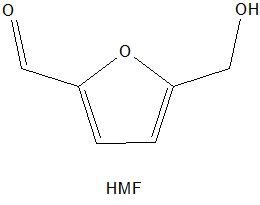
\includegraphics[width=0.5\textwidth]{../Bilder/HMF.jpg}
	\caption{Hydroxymethylfurfural}
	\label{fig:HMF}
\end{figure}
\newline
Eine Möglichkeit HMF in Honig zu bestimmen, ist die photometrische Methode nach WINKLER. Mittels einer Farbreaktion wird ein rot erscheinender Farbstoff erzeugt, der anschließend quantifiziert wird. Zur  Bestimmung des HMF-Gehalts wird zunächst die Methode, wie in dem Buch Lebensmittelanalytik~\cite{Lebensmittelanalytik} beschrieben, nachgestellt. Da in der zur Verfügung stehenden Methode lediglich ein Festfaktor zur Quantifizierung angegeben ist, wird zusätzlich eine Kalibrierreihe mit mehreren Messwerten durchgeführt. Des Weiteren wird die Methode auf Reproduzierbarkeit überprüft. Zur Ermittlung des Massenanteils an HMF werden mehrere Arten der Quantifizierung verwendet. Diese sind zum einen die Berechnung über den angegebenen Festfaktor, die Verwendung der erstellten Kalibriergeraden, sowie über Aufstockung einer Probe mit anschließender Standardadditionsberechnung. Es werden acht verschiedene Honige, ein Zuckerrübensirup und eine Invertzuckermischung, die bei Raumtemperatur aufbewahrt wurden, vermessen. Außerdem werden sechs der Honige für zehn Tage bei $60^\circ$ C gelagert und ein Anstieg des HMF-Gehalts nachgewiesen. Die Handhabung der Proben ist durch ihre Viskosität erschwert. Da der Honig viele verschiedene, zum Teil unlösliche Bestandteile enthält, wird diese Matrix vor der Bestimmung entfernt. Die verwendeten Chemikalien erfordern wegen ihrer gefährlichen Eigenschaften eine besonders sorgfältige Handhabung. Ihre Haltbarkeit ist auch bei korrekter Lagerung begrenzt. Der bei der Derivatisierung entstandene Farbstoff ist nicht stabil und zerfällt nach wenigen Minuten, deshalb muss jede Lösung zeitlich exakt vermessen werden.~\cite{Winkler}
\chapter{Planung}

\label{chap:Planung}
In diesem Kapitel sind Überlegungen zur Herangehensweise an die beschriebene Problemstellung aufgeführt. Diese Überlegungen umfassen sowohl die zu erwartende Probenmatrix als auch einzelne Schritte der Analyse wie z.B. die Fällung der störenden Bestandteile. Außerdem werden erste Berechnungen zur Erstellung einer Kalibriergeraden und den dazu nötigen Stammlösungen unternommen.

\section{Honig}
Honig besteht zum größten Teil aus Zucker. Zu etwa gleichen Teilen sind Fructose und Glucose mit je maximal 40\% enthalten. Andere Zucker wie Saccharose, Maltose und Melezitose sind je nach Zuckerart bis zu maximal 20\% enthalten. Da Honig jedoch ein Naturprodukt ist, kommen noch zahlreiche weitere Komponenten vor. So enthält Honig Enzyme, die in den bieneneigenen Drüsen produziert werden. Drei der wichtigsten Enzyme sind die Invertase, die Amylase und die Glucoseoxidase. Invertase spaltet Saccharose in Glucose und Fructose, während die Amylase zur Spaltung der Stärke in Maltose dient. Glucoseoxidase wandelt in wässriger Lösung und in Verbindung mit Luftsauerstoff, Glucose in Wasserstoffperoxyd um und entwickelt damit eine antibakterielle Wirkung. Des weiteren ist das in dieser Analyse bestimmte Hydroxymethylfurfural ein Bestandteil, der sich bei der Zersetzung von Fructose unter Wärme und Säureeinfluss bildet. Im Spurenbereich finden sich noch Vitamine, Hormone und Mineralstoffe im Honig. Außerdem kann die Aminosäure Prolin darin nachgewiesen werden. Der Gehalt beträgt je nach Reifegrad zwischen 250 und 550mg/kg.\\
Honig hat einen leicht sauren pH-Wert, der meist zwischen 3,2 bis 5,4 liegt. Ursache dafür sind im Honig vorkommende organische Säuren, hauptsächlich sind dies Ameisensäure und Zitronensäure. Der Geschmack mag vom hohen Zuckergehalt überlagert werden, trotzdem hat Honig korrosive Eigenschaften.\\
Liegt der Honig als Rohprodukt vor und wurde nicht gefiltert, sind in ihm auch noch einige feste Bestandteile enthalten wie Pollenkörner, Pilzsporen, Algen und auch tierische Bestandteile wie Bienenhaare. Zuletzt findet sich auch ein nicht unerheblicher Anteil an Wasser im Honig. Dieser kann zwischen 15 bis 19\% betragen. Ist der Wassergehalt erhöht, kann es zur Gärung kommen und der Honig verdirbt. Ist er zu niedrig kristallisiert der Zucker aus und der Honig wird inhomogen.\\
Alle diese Bestandteile können bei der Photometrischen Analyse problematisch sein, da sie entweder die gesamte Lösung trüben oder evtl. eine Absorptionsbande im benötigten Bereich bei 550nm aufweisen. Deshalb ist es ratsam in einem vorbereitenden Schritt die meisten Matrixbestandteile abzutrennen.~\cite{LWG}
\begin{figure}[htbp]
	\centering
		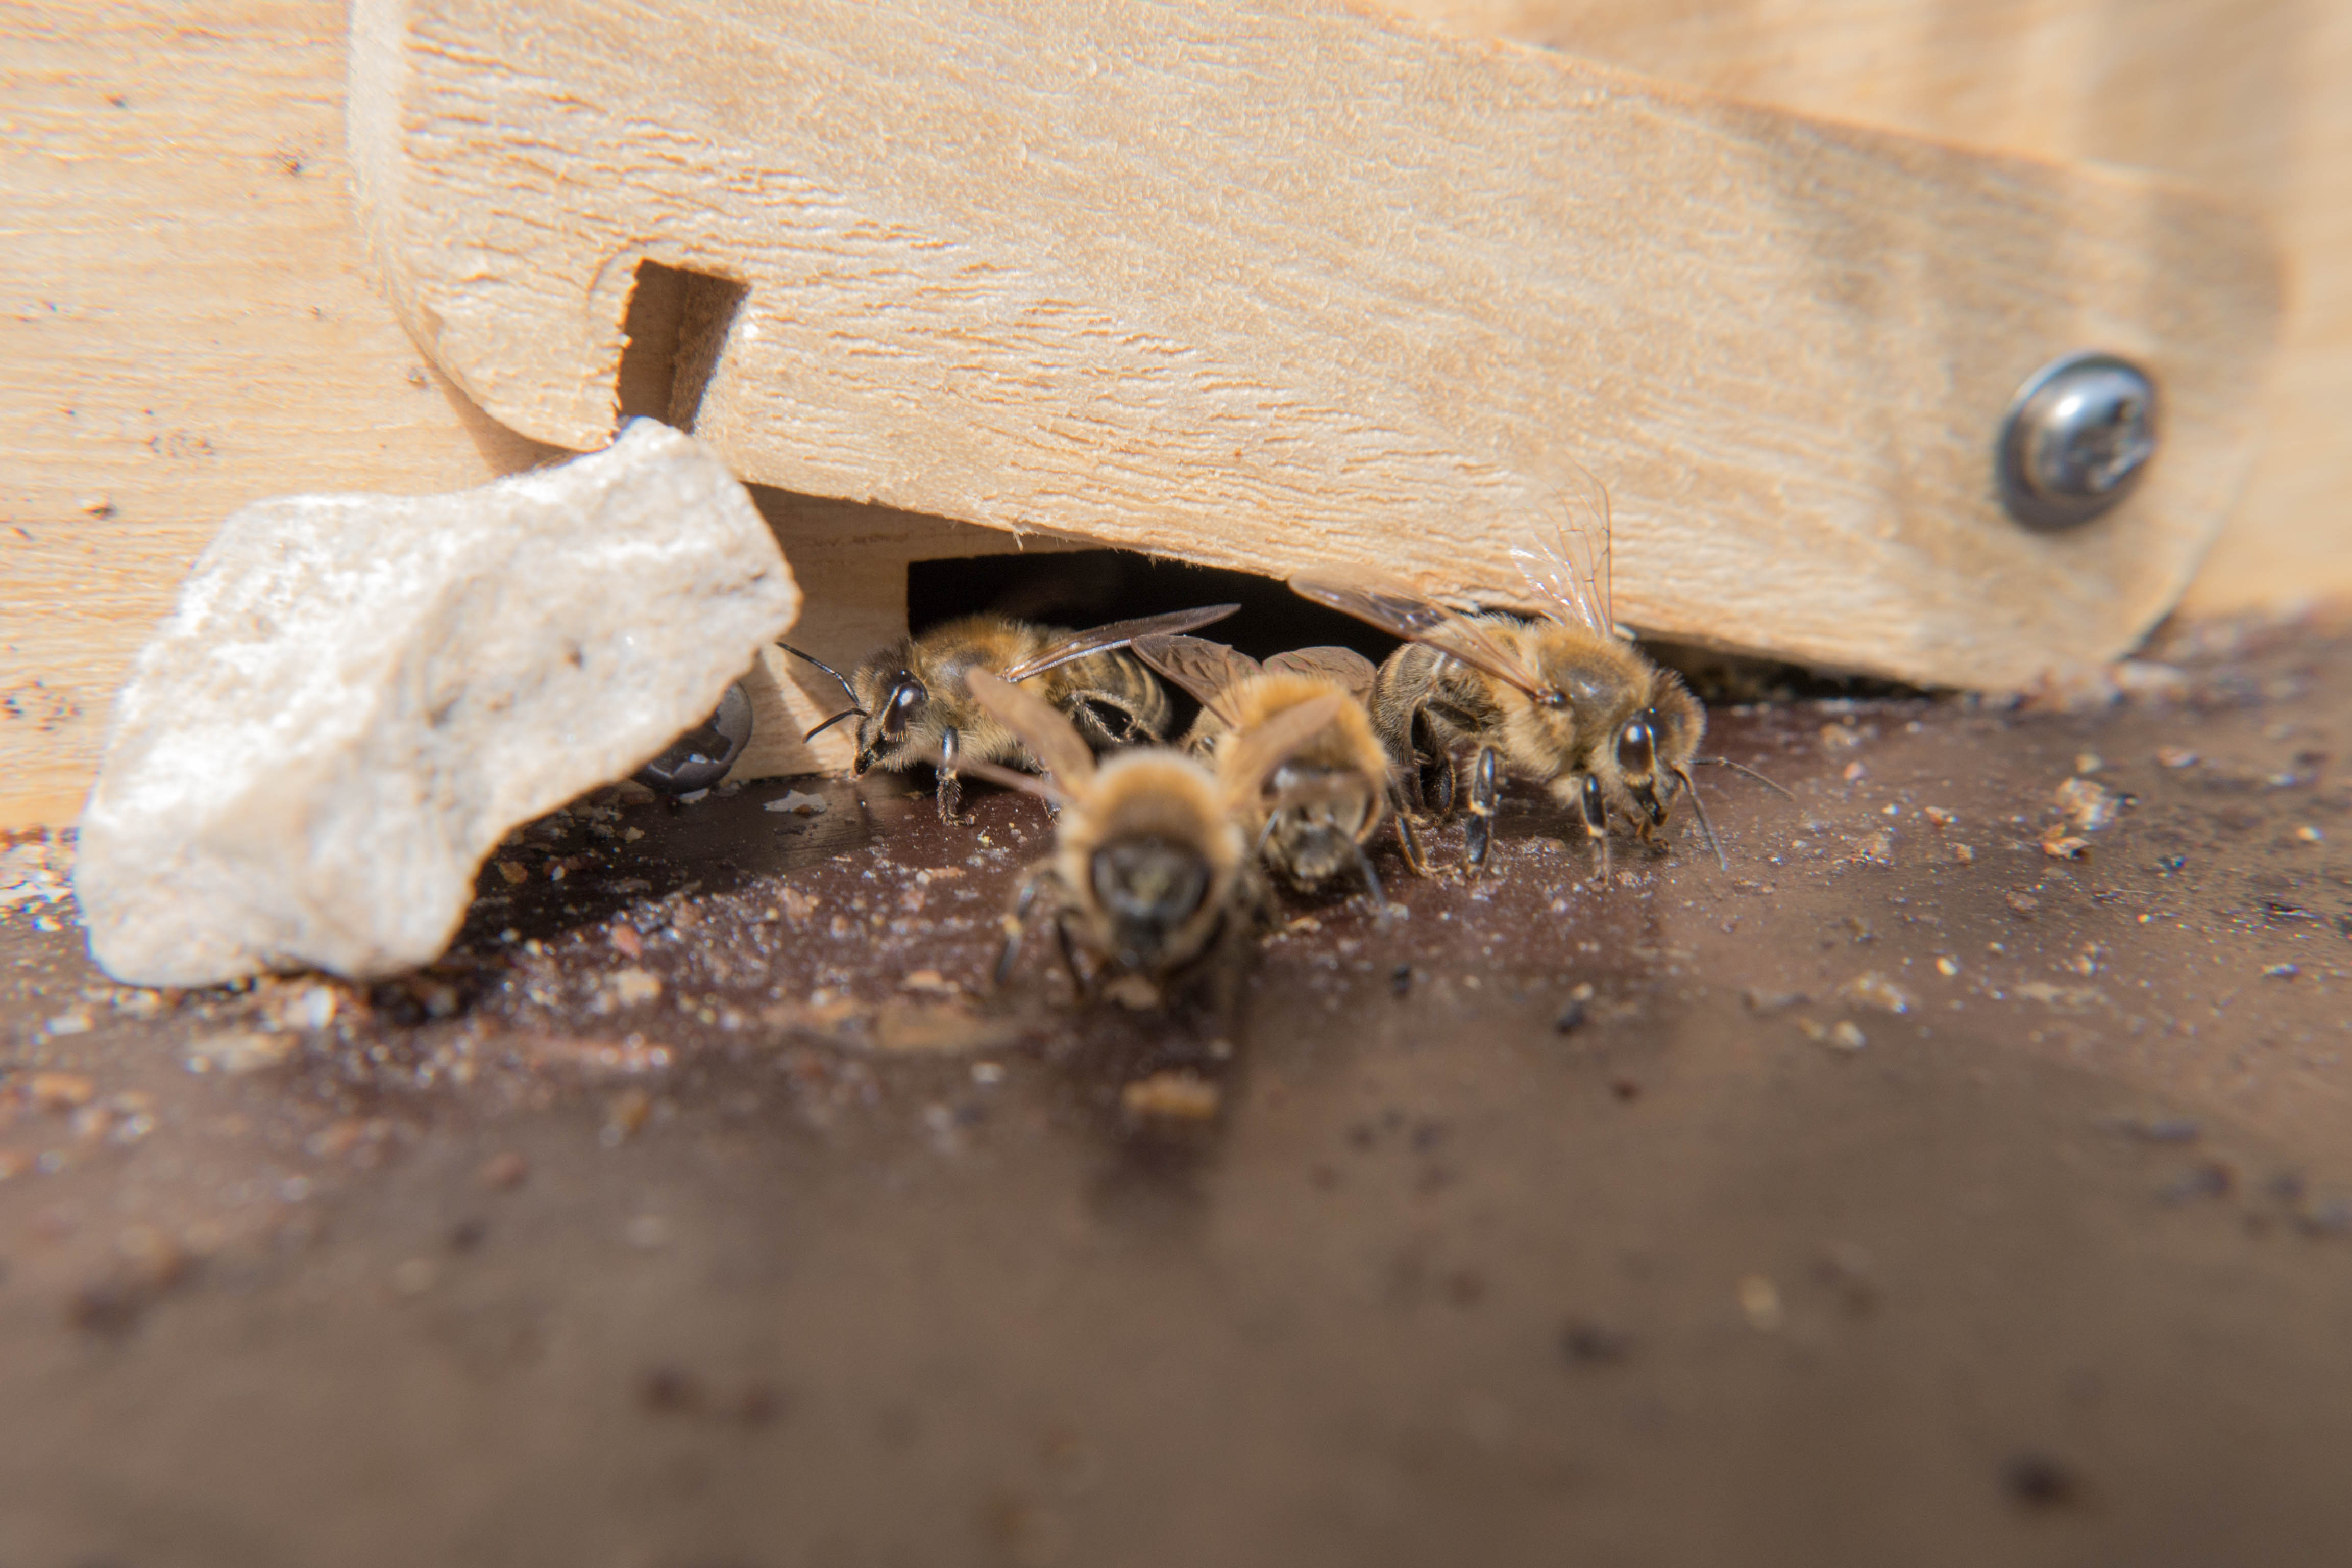
\includegraphics[width=1.00\textwidth]{../Bilder/P1050729.jpg}
	\caption{Bienen}
	\label{fig:Bienen}
\end{figure}


\section{Bildung von HMF}

Wird Honig über lange Zeit gelagert oder hohen Temperaturen ausgesetzt, so bildet sich aus der enthaltenen Fructofuranose unter Wasserabspaltung Hydroxymethylfurfural.~\cite{HMF} Dies verdeutlicht die folgende Reaktionsgleichung \ref{fig:HMFEntstehung}. 
  
\begin{figure}[htbp]
	\centering
		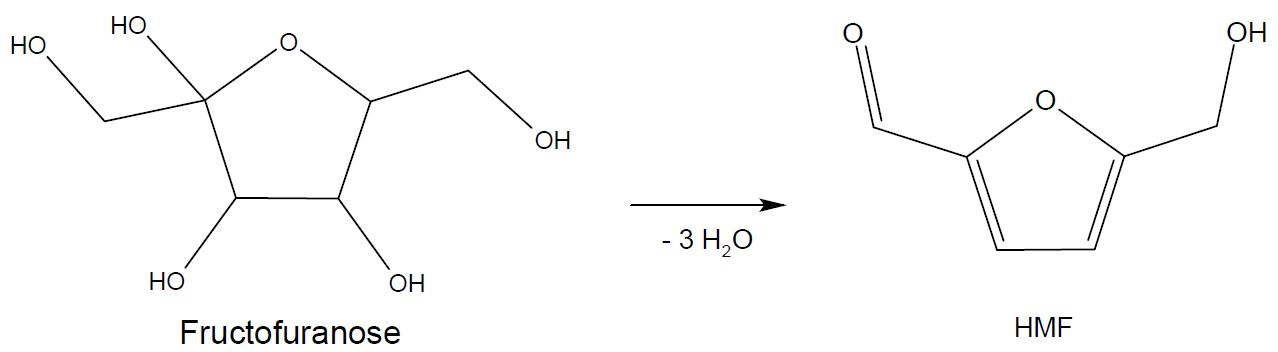
\includegraphics[width=1.00\textwidth]{../Bilder/HMFEntstehung.JPG}
	\caption{Reaktionsgleichung Fructofuranose}
	\label{fig:HMFEntstehung}
\end{figure}

\section{Nachweis nach Winkler}

O. Winkler veröffentlichte im September 1955 in der ``Zeitschrift für Lebensmittel-Untersuchung und -Forschung'' einen Bericht über eine neue Methode HMF spektroskopisch in Honigen nachzuweisen. Dieser Nachweis basiert auf Furfurol-Farbstoffen, die von Boehm und Grohnewald beschrieben wurden und auf der von Akabori dargestellten Reaktion von Furfuraldehyden mit Barbitursäure und Anilin. Winkler ersetzte das Anilin durch p-Toluidin, ein kernsubstituiertes Derivat, das die gleiche Reaktion mit HMF und Barbitursäure zeigt. Durch Zugabe von Eisessig in die isopropanolische p-Toluidinlösung konnte die Empfindlichkeit der Reaktion verbessert werden. P-Toluidin wird heute als potentiell krebserzeugend eingestuft und muss deshalb mit größter Vorsicht im Abzug und mit der nötigen persönlichen Schutzausrüstung gehandhabt werden.\\
Der entstehende rote Farbstoff, der in der folgenden Reaktionsgleichung \ref{fig:Farbreaktionsgleichung2} dargestellt ist, absorbiert bei 550nm das sichtbare Licht und erreicht drei bis vier Minuten nach Zugabe des letzten Reaktionsmittels seine höchste Intensität. Danach zerfällt der Farbstoff wieder. Nach O. Winkler ist die Linearität der Messung zwischen 5 und 300ppm HMF gegeben.~\cite{Winkler}

\begin{figure}[htbp]
	\centering
		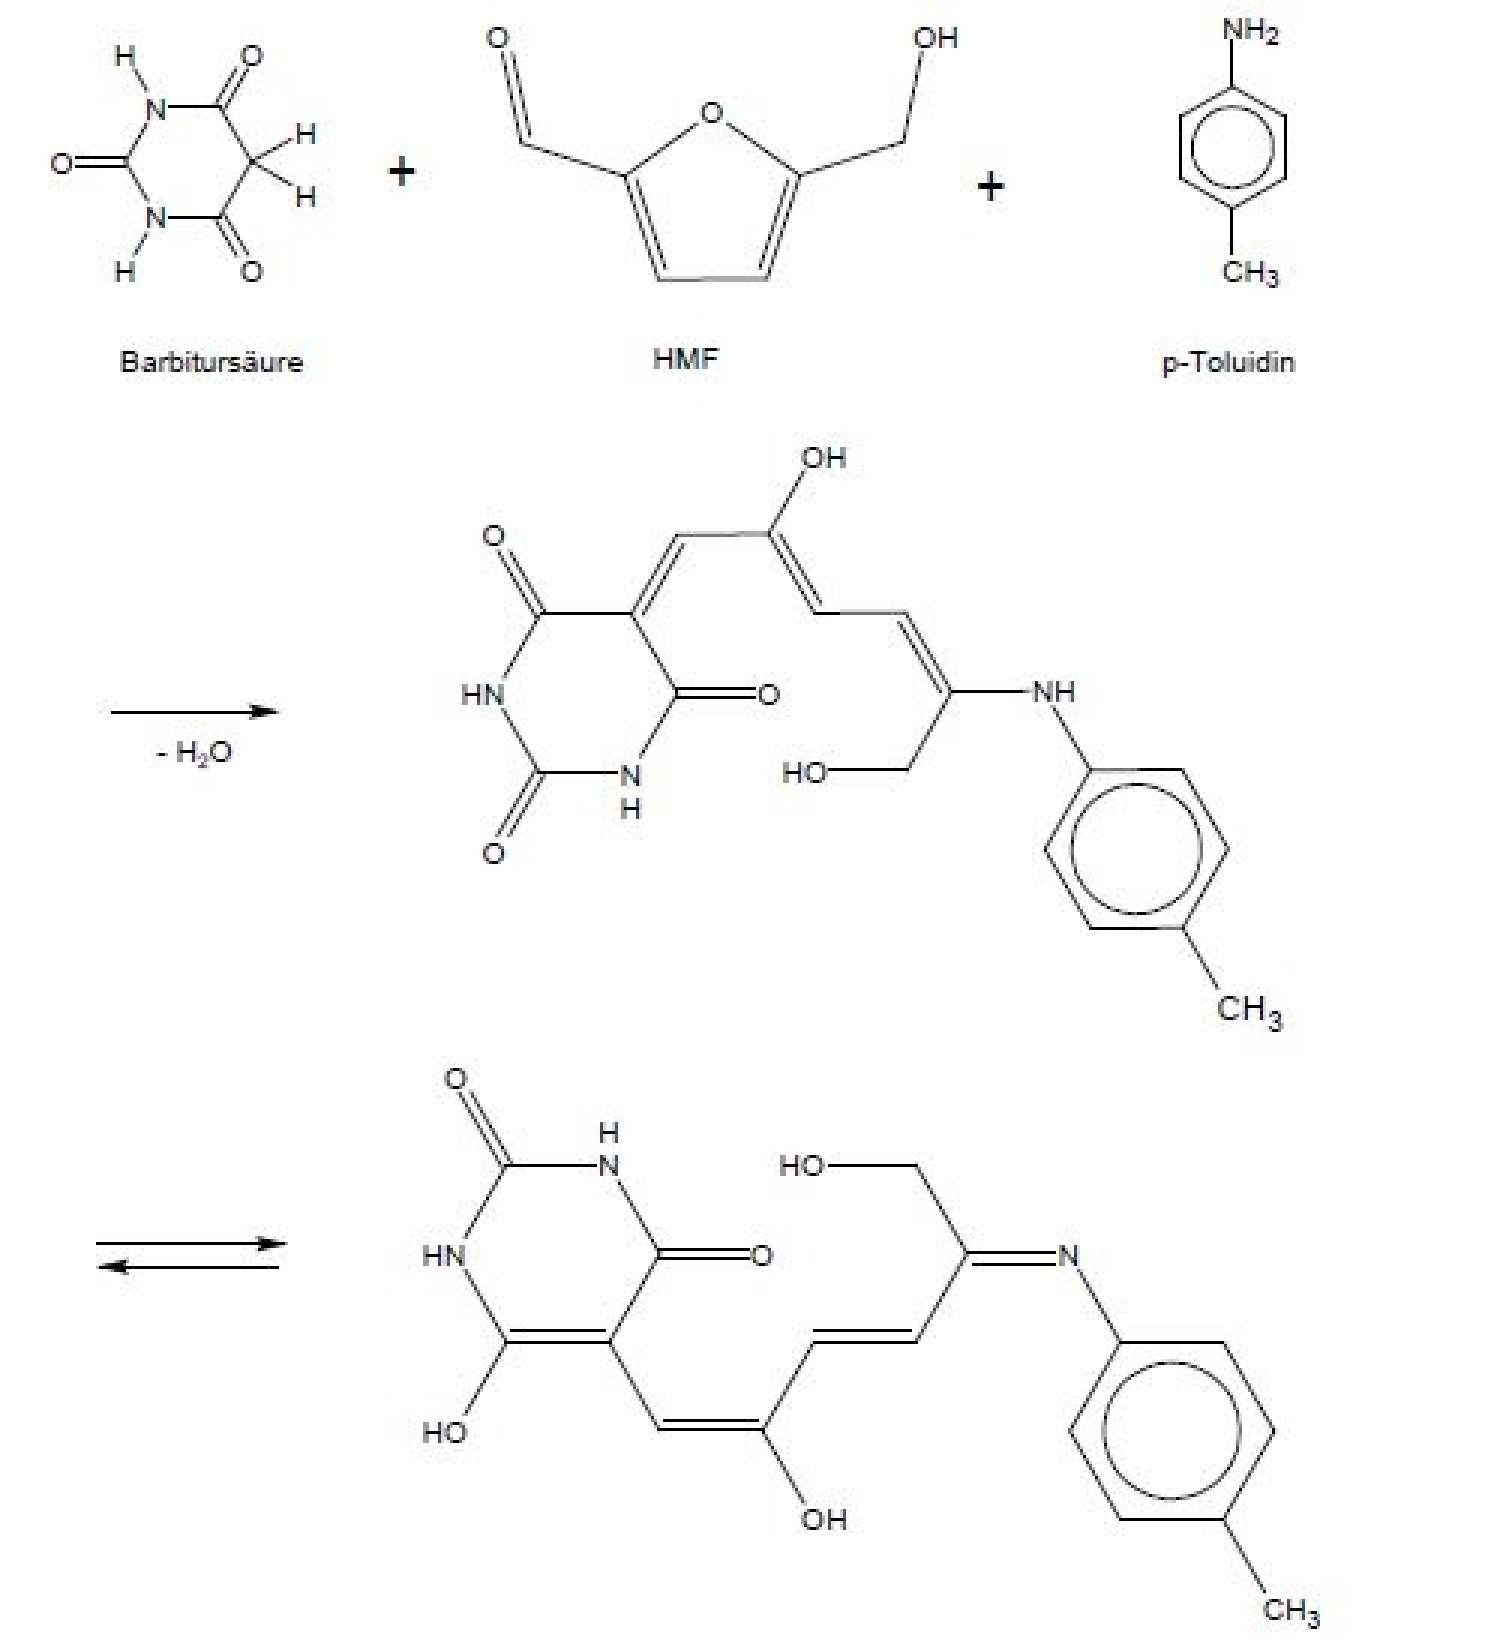
\includegraphics[width=1.00\textwidth]{../Bilder/Farbreaktionsgleichung2.pdf}
	\caption{Reaktionsgleichung HMF}
	\label{fig:Farbreaktionsgleichung2}
\end{figure}

\section{Alternative Nachweismethoden}

Neben dem HMF-Nachweis nach WINKLER gibt es noch weitere Methoden um HMF in zuckerhaltigen Produkten nachzuweisen.\\
Es gibt zum Beispiel die Möglichkeit das HMF mit Diethylether aus der Probe zu extrahieren und mit einer Resorcinlösung, auch Seliwanoff-Reagenz genannt, als roten Farbstoff sichtbar zu machen. Da das Resorcin auch mit der vorhandenen Fructose reagiert, ist für einen korrekten Nachweis eine saubere Extraktion unbedingt notwendig. Allerdings sind sowohl das Resorcin als auch der Diethylether als gesundheitsschädlich eingestuft und der Versuch muss im Abzug durchgeführt werden.~\cite{Resorcinnachweis} Hierbei handelt es sich um den sogenannten Fieheschen Nachweis.~\cite{Winkler}\\
Weiterhin zeigt HMF in wässriger Lösung bei 282nm ein Absorptionsmaximum. Über diesen und zwei weitere Messpunkte bei 245 und 325nm lässt sich nach Schou und Abildgaard der HMF-Gehalt in einer Probe berechnen. Allerdings absorbiert zum Beispiel Honig bei diesen Wellenlängen durch seine Matrixbestandteile ebenfalls Licht. Dies verfälscht das Messergebnis. Durch Zugabe der Carrez-Lösungen I und II können die störenden Bestandteile zu einem Großteil entfernt werden und die Richtigkeit des Ergebnisses verbessert werden.~\cite{Winkler}
Alternativ kann HMF auch per Gaschromatographie oder HPLC bestimmt werden. Hierfür müssen die Proben in einer säulengängigen Form vorliegen und die Methoden für eine Quantifizierung mit einem HMF-Standard kalibriert werden.~\cite{Patent}
Alle hier genannten HMF-Nachweise sind mit hohem chemischem und apparativem Aufwand verbunden. Außerdem sind die verwendeten Chemikalien gesundheitsschädlich oder sogar giftig und müssen deshalb mit größter Vorsicht gehandhabt werden. Aus diesen Gründen wurde von Merck ein einfacher Schnelltest entwickelt. Dieser erfolgt mit Teststäbchen, die mit zwei Reaktionslösungen belegt sind. Die Stäbchen müssen nur in die Probe eingetaucht und dann in einem Reflektometer vermessen werden. Hierbei erfolgt die Farbreaktion auf dem Teststäbchen. Das Gerät kann HMF-Konzentrationen zwischen 1 und 60mg/L erfassen. Höher konzentrierte Proben müssen verdünnt und das Messergebnis mit dieser Verdünnung verrechnet werden. Die Farbreaktion ist zeitabhängig, deshalb muss auch hierbei die Reaktionszeit genau eingehalten werden.~\cite{Merck}

\section{Bedeutung von HMF}
In den 1950er Jahren wurde HMF erstmals in Lebensmitteln nachgewiesen. Es besitzt kein relevantes toxisches Potential. Die lethale Dosis bei oraler Einnahme für Ratten beträgt 3100mg/kg. Jedoch ist die kanzerogene Wirkung von HMF weitestgehend unklar. Zwar kann aus bisher vorliegenden Studien keine Relevanz bezüglich krebserzeugender oder erbgutschädigender Wirkung beim Menschen festgestellt werden, jedoch ist die Bedeutung der Stoffwechselabbauprodukte und deren Wirkung bei der Entstehung von Darmkrebs nicht restlos aufgeklärt. Ebenfalls eine kurzzeitig angenommene krebsvorbeugende Wirkung konnte nicht bestätigt werden.
\\
Die Konzentration von HMF in Honig ist selbst bei relativ hohen Gehalten eher gering im Vergleich zu anderen Lebensmitteln. In Honig befindet sich, nach Daten des Bundesinstituts für Risikobewertung, ein mittlerer HMF-Gehalt von 9,1mg/kg. Zum Vergleich besitzt Mehrfruchtnektar einen mittleren Gehalt von 40,9mg/kg und Saft aus Trockenpflaumen sogar einen mittleren Gehalt von 1022,1mg/kg. Der Massenanteil an HMF in Honig ist somit primär der Indikator für Frische und die korrekte Lagerung. So gelten für Honig in Deutschland verschiedene Bestimmungen, die den maximalen Massenanteil an HMF vorgeben. Nach der deutschen Honigverordnung ist in deutschem Honig eine maximale Obergrenze von 40mg/kg HMF zulässig. In Honig aus tropischen Regionen ist sogar ein Gehalt von 80mg/kg noch erlaubt. Deutlich strenger sind die Kriterien, die der Deutsche Imkerbund an Honige anlegt, die das Gütesiegel ``echter deutscher Honig'' tragen wollen. Hierfür liegt die Obergrenze für HMF bei 15mg/kg und für niedrig enzymatischen Honig sogar nur bei 5mg/kg.
\\
Eine direkte Verwendung findet HMF als Aromastoff in Lebensmitteln als Bestandteil von Raucharoma. Jedoch wird HMF derzeit neu betrachtet und eventuell neu bewertet.~\cite{BfR}

\section{Funktionsweise eines UV/VIS-Spektroskops}

\begin{figure}[htbp]
	\centering
		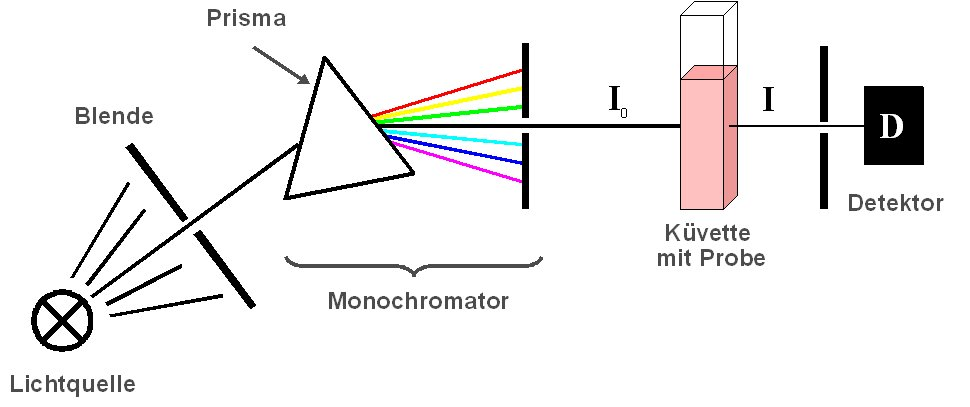
\includegraphics[width=1.00\textwidth]{../Bilder/Einstrahlspektrometer.jpg}
	\caption{Schematischer Aufbau eines Einstrahl-Absorptionsspektrometers \cite{Schema}}
	\label{fig:Einstrahlspektrometer}
\end{figure}

Die UV/VIS-Spektrometrie gehört zur Absorptionsspektroskopie. Dabei wird die Konzentration
eines Lösungsbestandteils (= Analyt) in einer optisch klaren Lösung über die Absorption
eines möglichst monochromatischen Lichtstrahls bestimmt.\\
Aus dem polychromatischen Licht einer Lichtquelle wird mittels einer Blende ein einzelner
Lichtstrahl abgetrennt und auf ein Prisma gelenkt. Dort wird er in einzelne monochromatische
Lichtstrahle aufgetrennt. Ein Lichtstrahl einer bestimmten Wellenlänge wird
durch eine Küvette, die mit der Probelösung gefüllt ist, geleitet. Ein Teil des Lichtstrahls wird
durch die Probe absorbiert. Das restliche austretende Licht wird detektiert und die Extinktion
daraus berechnet.
\begin{figure}[htbp]
	\centering
		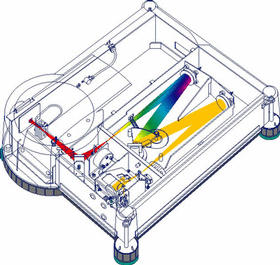
\includegraphics[width=1.00\textwidth]{../Bilder/AufbauSpektrometer.jpg}
	\caption{Schematischer Aufbau Varian Cary 50 Scan UV/VIS-Spektrometer \cite{UV-VIS}}
	\label{fig:AufbauSpektrometer}
\end{figure}

Das UV-VIS Spektrometer Varian Cary® 50 besitzt eine Xenon-Blitzlampe als Lichtquelle, die dem Benutzer dieses
Spektralphotometers viele Vorteile bietet. Das Instrument wird direkt über einen Computer mit
der Cary Win UV-Software gesteuert. Für verschiedene Benutzeranforderungen ist eine Auswahl
an Softwarepaketen erhältlich.
\begin{figure}[htbp]
	\centering
		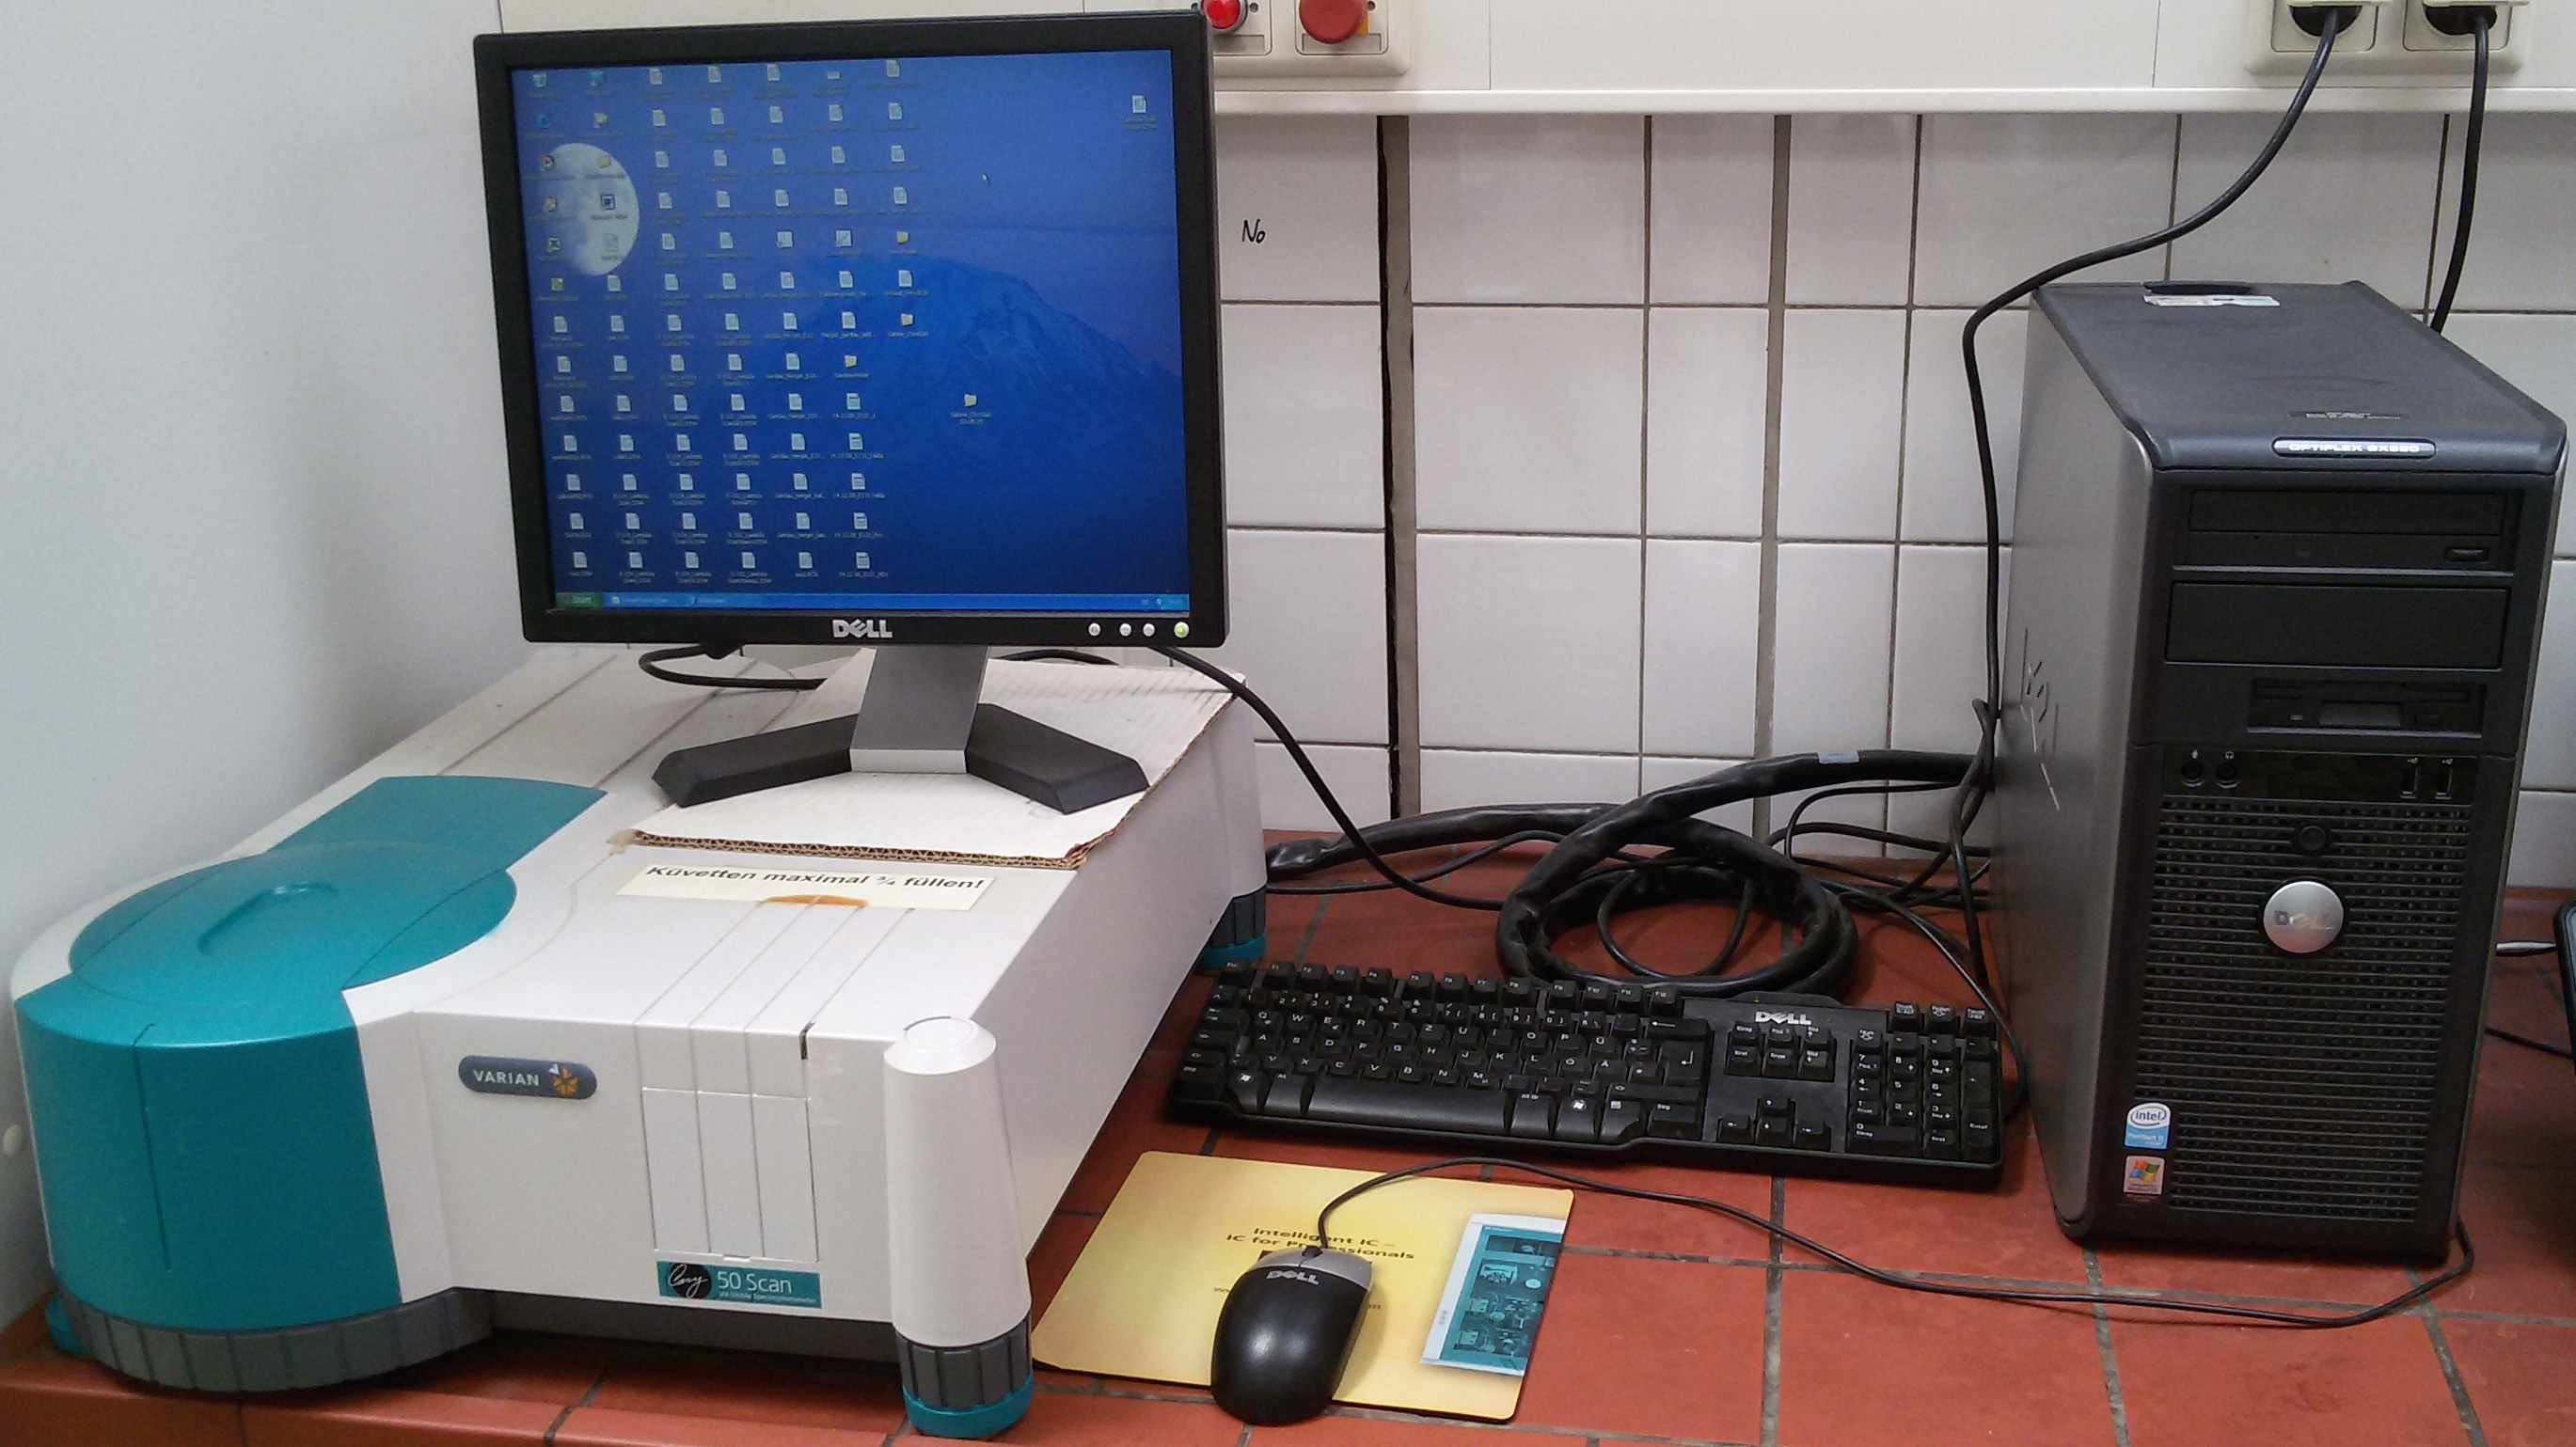
\includegraphics[width=1.00\textwidth]{../Bilder/20150504_140611.jpg}
	\caption{Varian Cary 50 Scan UV/VIS-Spektrometer }
	\label{fig:Spektrometer}
\end{figure}

\section{Funktion Carrez-Lösung}
Da die Honiglösung noch viele trübende Bestandteile enthält, muss sie mit der Carrez-Klärung von Kolloiden getrennt werden. Dazu wird eine Lösung aus gelbem Blutlaugensalz (Carrez I) und eine Lösung aus Zinkacetat (Carrez II) verwendet. Beide Lösungen müssen zu gleichen Teilen der Probelösung zugegeben werden. Dabei entsteht Kalium-Zink-hexacyanoferrat(II) $(K_{2}Zn_{3}[Fe(CN)_{6}]_{2})$, das die meisten kolloiden Trübstoffe aus der Lösung entfernt. Nach O. Winkler findet eine Absorption des enstehenden Farbstoffs mit dem Klärmittel nach zahlreichen Versuchen nicht statt. Durch Filtration können die ausgefallenen Bestandteile abgetrennt und verworfen werden. Das klare Filtrat kann weiter verarbeitet werden.~\cite{Winkler}

\section{Organisation des Abschlussprojektes}
Während der Recherchen zur Durchführung unseres Abschlussprojektes entdeckten wir, dass die beiden Reaktionslösungen (p-Toluidinlösung und Barbitursäure) in der benötigten Konzentration im Chemikalienhandel erhältlich sind. Über die Chemikalienbeschaffung der BASF SE konnten sowohl der benötigte HMF-Standard als auch die beiden Reaktionslösungen bestellt werden. Somit entfällt das Ansetzen der beiden Lösungen während des Praktikums. Es konnte von Seiten des Herstellers keine Aussage über die Haltbarkeit der p-Toluidinlösung nach Öffnung der Flasche getroffen werden. Die selbst angesetzte Lösung wäre nur drei Tage haltbar gewesen. Die restlichen Chemikalien stellte die Berufsschule zur Verfügung. \\
\begin{figure}[tbp]
	\centering
		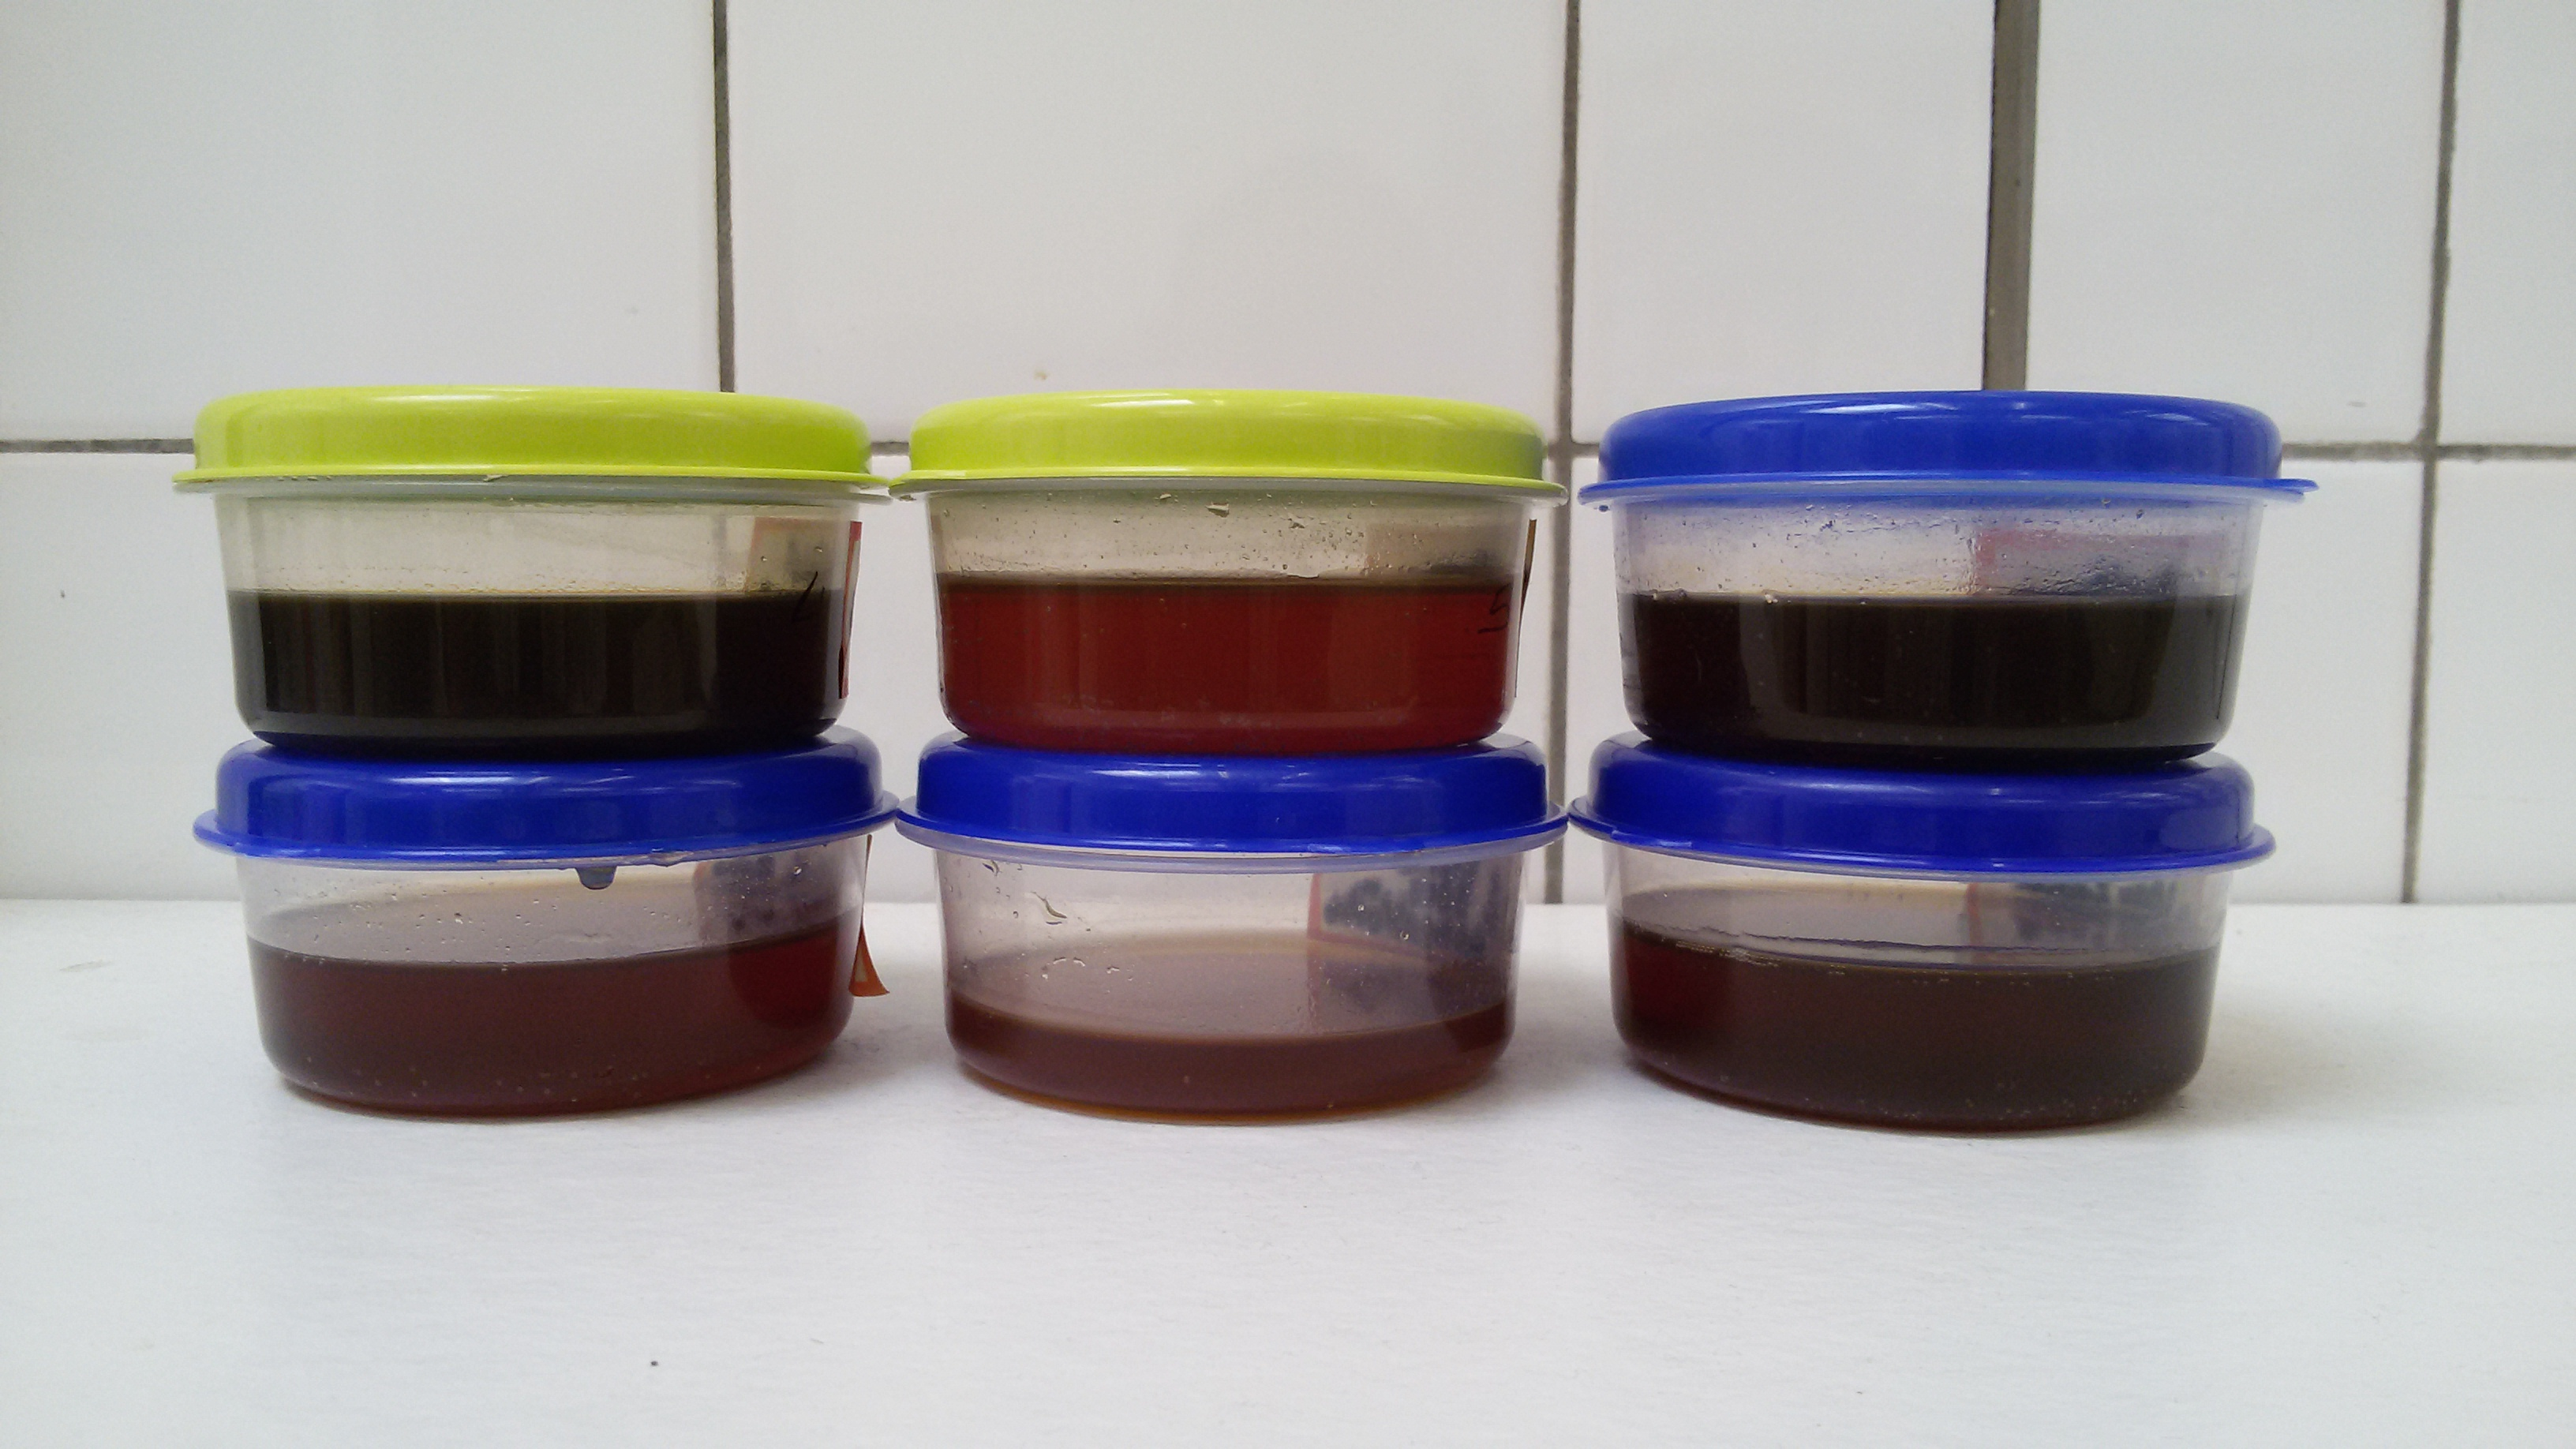
\includegraphics[width=1.00\textwidth]{../Bilder/20150504_141528.jpg}
	\caption{Honigproben für Lagertest}
	\label{fig:Lagertest}
\end{figure}
Zehn Tage vor dem zweiten Praktikumstag wurden die zugekauften Chemikalien im Chemikalienkühlschrank der Biologie in der BBSN Ludwigshafen verwahrt. Am gleichen Tag wurden auch die sechs Honigproben für den Lagertest abgefüllt. Sie wurden in einem Wärmeschrank der Biologie bei einer Temperatur von $60^\circ$ C gelagert.\\
Für die Durchführung des Abschlusspraktikums wurden anderthalb Praktikumstage angesetzt. Auf Grund von Problemen während des Praktikums wurde ein zusätzlicher Tag benötigt. \\
Für die vier Stunden des ersten Praktikumstages wurde das Ansetzen der beiden Carrez-Lösungen, eine erste Probemessung mit einer Honigprobe ohne und mit Temperaturlagerung und das Erstellen der Kalibriergeraden vorgesehen.\\
Am zweiten Praktikumstag sollten die Proben vermessen werden. Da hierbei erkannt wurde, dass der Farbstoff nach einiger Zeit zerfällt, wurde ein weiterer Praktikumstag eingeplant.\\
Während des dritten Tages wurde die Kalibrierung wiederholt und eine Sechsfachanalyse, sowie eine Aufstockung einer Honigprobe mit HMF durchgeführt.\\

\section{Berechnungsgrundlagen}
Für die Berechnung der notwendigen Kalibrierlösungen berücksichtigen wir, dass in den Versuchen von WINKLER die Extinktion von HMF zwischen 5 - 300mg/kg einen linearen Verlauf aufweist. Um die Möglichkeit eines zufälligen Wägefehlers zu minimieren, werden zwei Stammlösungen mit verschiedenen Konzentrationen angesetzt. Auf Grund der benötigten Kalibrierung mit 5mg/kg, müssen die Stammlösungen noch entsprechend verdünnt werden. Für die kleinste und größte Kalibration werden folgende Mengen HMF benötigt:

	\[w[mg/kg]=\frac{ m(HMF) }{ m(Gesamt) }\]
	
Die Formel wird nach m(HMF) umgestellt.

	\[m(HMF)=w[mg/kg]*m(Gesamt)\]
	
Für 5mg/kg bedeutet dies:
	
	\[0,05mg=5mg/kg*0,01kg\]
	
Und für 300mg/kg:

	\[3,00mg=300mg/kg*0,01kg\]
	
Alle Massenanteile beziehen sich auf eine ideale Einwaage von 10,00g und ein Endvolumen von 50ml.
Da die Kalibriergerade der Software die Massenkonzentration in mg/L ausgibt, werden die Gehalte zusätzlich entsprechend umgerechnet:

\[\beta=\frac{ m(HMF) }{ V }\]

Das bedeutet bei 5mg/kg:

\[1mg/L=\frac{ 0,05mg }{ 0,05L }\]

Und wieder für 300mg/kg:

\[60mg/L=\frac{ 3,00mg }{ 0,05L }\]

Wir erwarten vor allem Gehalte zwischen 5 bis 100mg/kg HMF in unseren Proben, deshalb liegen die meisten unserer Kalibrierpunkte eher in diesem Konzentrationsbereich.
In Tablle \ref{tab:Stammlösungen} sind die Daten für die Stammlösungen aufgelistet:

\begin{table}[htbp]
	\centering
	\caption{Stammlösungen}
		\begin{tabular}{l|c|c|l}
			Bezeichnung & m(HMF) in mg & Konzentration in mg/L & Bemerkung\\
			\hline
			Stammlösung 1 & 50 & 5000  & in 10ml Messkolben\\
			\hline
			Stammlösung 1.1 & 5 & 50 & 1ml SL1 in 100ml\\
			\hline
			Stammlösung 2 & 150 & 15000 & in 10ml Messkolben\\
			\hline
			Stammlösung 2.1 & 15 & 150 & 1ml SL2 in 100ml\\
		\end{tabular}
		\label{tab:Stammlösungen}
\end{table}

Aus den Stammlösungen werden die in der folgenden Tabelle \ref{tab:IdealeKalibrierfaktoren} eingetragenen Faktoren hergestellt:

\begin{table}[htbp]
	\centering
	\caption{Ideale Kalibrierfaktoren}
		\begin{tabular}{L{0.15\linewidth}|C{0.15\linewidth}|C{0.17\linewidth}|C{0.17\linewidth}|L{0.22\linewidth}}
			Bezeichnung & m(HMF)\newline in mg & Konzentration\newline in mg/L & Massenanteil\newline in mg/kg & Bemerkung\\
			\hline
			Faktor 1 & 0,05 & 1,00  & 5 & 1ml SL1.1 in 50ml\\
			\hline
			Faktor 2 & 0,15 & 3,00  & 15 & 1ml SL2.1 in 50ml\\
			\hline
			Faktor 3 & 0,25 & 5,00  & 25 & 5ml SL1.1 in 50ml\\
			\hline
			Faktor 4 & 0,50 & 10,00 & 50 & 10ml SL1.1 in 50ml\\
			\hline
			Faktor 5 & 1,50 & 30,00 & 150 & 10ml SL2.1 in 50ml\\
			\hline
			Faktor 6 & 3,00 & 60,00 & 300 & 20ml SL2.1 in 50ml\\
		\end{tabular}
		\label{tab:IdealeKalibrierfaktoren}
\end{table}

Allen diesen Konzentrationen liegen idealen Berechnungen zugrunde. Die reellen Einwaagen sind im Kapitel~\ref{chap:Durchführung} Durchführung zu finden.

\chapter{Durchführung}

\label{chap:Durchführung}

Für die Kalibrierung und die Probenvermessung müssen verschiedene Reaktionslösungen angesetzt werden, die einerseits die Matrixeinflüsse verhindern und andererseits für die Farbreaktion benötigt werden. Im folgenden Kapitel sind die verwendeten Chemikalien und Geräte aufgelistet, sowie der genaue Arbeitsablauf gemäß der Vorschrift aus dem Buch Lebensmittelanalytik~\cite{Lebensmittelanalytik} beschrieben.

\section{Verwendete Chemikalien}

Um störende Matrixbestandteile der Honigproben vorab zu entfernen, werden die Carrez-Lösungen I und II benötigt. Die für die Farbreaktion verwendeten Reaktionslösungen können im Chemikalienhandel erworben werden. Dies gilt ebenfalls für die Reinsubstanz HMF, die für die Kalibrierlösungen und die Aufstockung benutzt wird. In der nachfolgenden Tabelle \ref{tab:Chemikalienliste} sind alle benötigten Chemikalien aufgelistet.

\begin{table}[htbp]
    \centering
        \caption{Chemikalienliste}
        \begin{tabular}{L{0.18\linewidth}|C{0.13\linewidth}|C{0.1\linewidth}|c|c|c} 
            Chemikalie & CAS/ Artikel-Nr. & Gefahren-symbol & Reinheit & Hersteller & Lot-Nr.\\
            \hline
            Hydroxymethyl-furfural & 67-47-0 & 
\includegraphics{../Bilder/Ausrufezeichen.jpg} & 97\% & Alfa Aesar & 10189124\\
            \hline
            p-Toluidin-lösung & 18686.2700 & 
\includegraphics{../Bilder/Flamme.jpg} 
\includegraphics{../Bilder/Gesundheitsgefahr.jpg} 
\includegraphics{../Bilder/Ausrufezeichen.jpg} & 100g/L & Bernd Kraft & 1632697\\
            \hline
            Barbitursäure-lösung & 18685.2700 & - & 5g/L & Bernd Kraft & 1632696\\
            \hline
            Kaliumhexa-cyanoferrat-(II)-Trihydrat & 14459-95-1 & - & $\geq99\%$ & Sigma-Aldrich & SZBC2230V\\
            \hline
            Zinkacetat-Dihydrat & 5970-45-6 & 
\includegraphics{../Bilder/Ausrufezeichen.jpg} 
\includegraphics{../Bilder/Umwelt.jpg} & $\geq99,5\%$ & Merck & A0180402 142\\
            \hline
            VE-Wasser & & & & &
        \end{tabular}
    \label{tab:Chemikalienliste}
\end{table}

\begin{figure}[htbp]
    \centering
        \subfigure[p-Toluidinlösung]{
    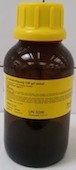
\includegraphics[]{../Bilder/20150504_140919.jpg}}
        \subfigure[Barbitursäurelösung]{
        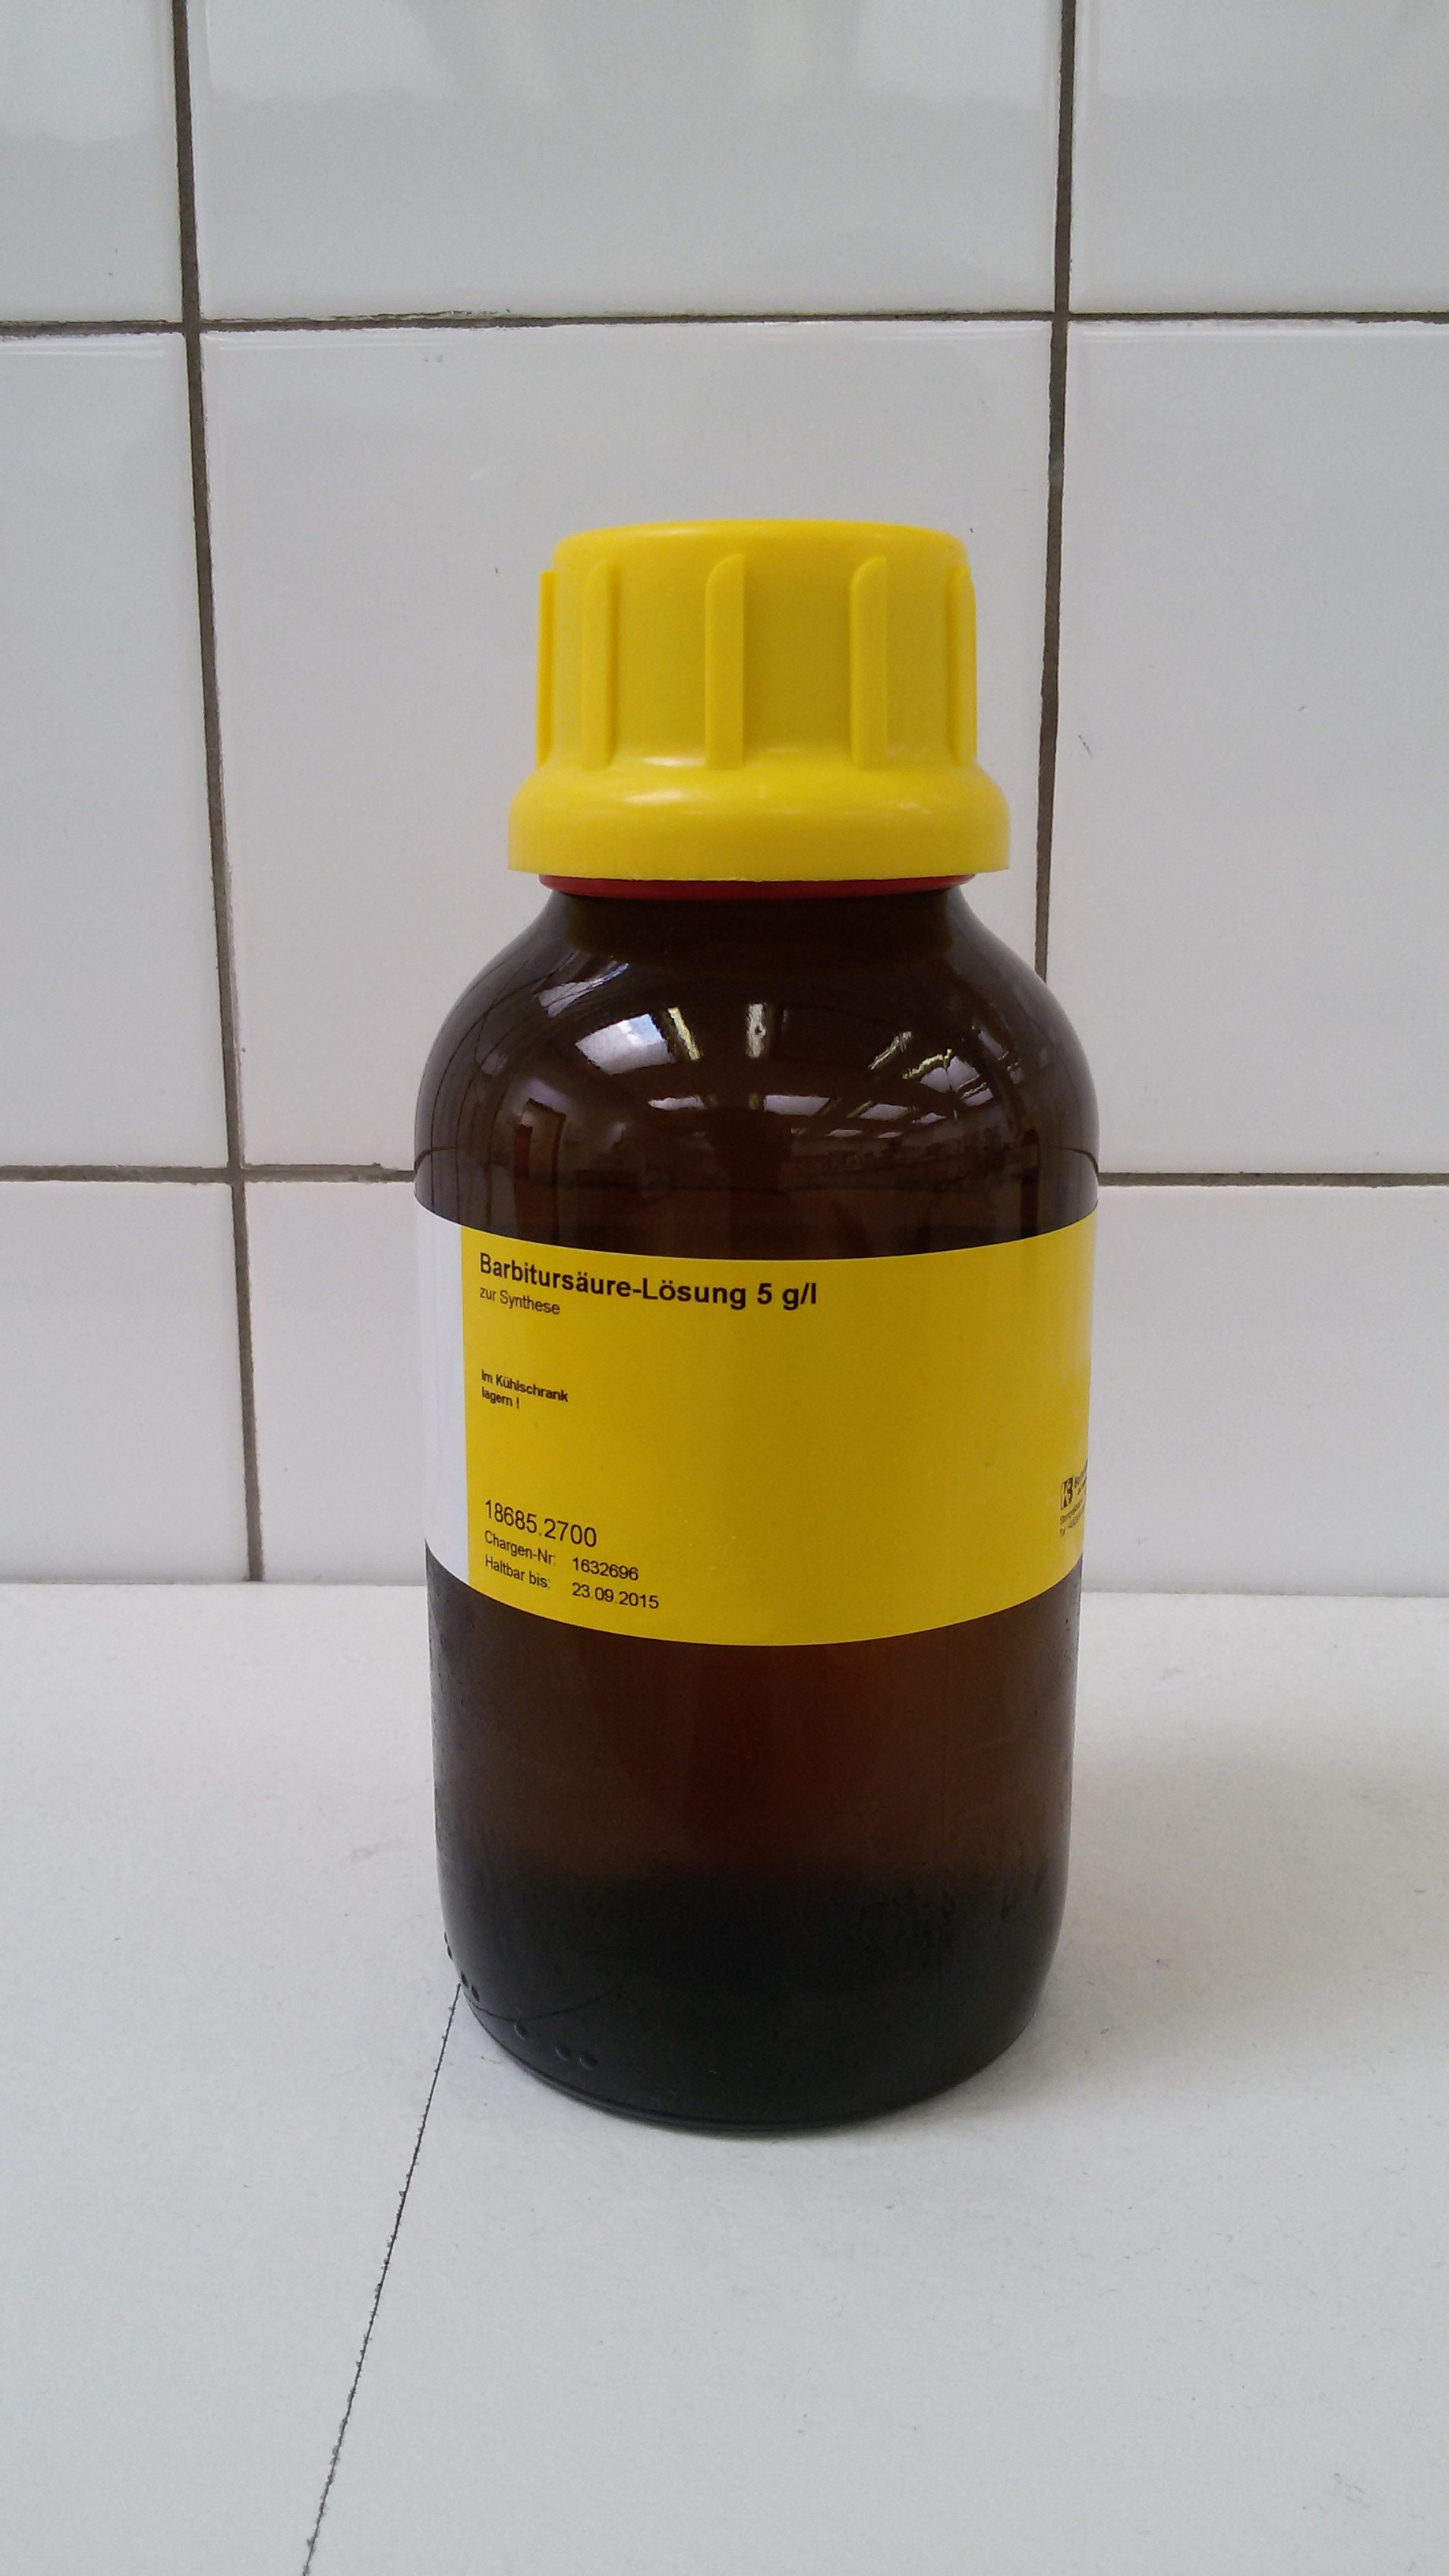
\includegraphics[]{../Bilder/20150504_140946.jpg}}
        \subfigure[\small Kaliumhexa-cyano-ferrat-(II)-Trihydrat]{
        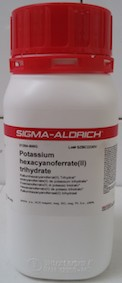
\includegraphics[]{../Bilder/20150504_141221.jpg}}
        \subfigure[Zinkacetat-Dihydrat]{
        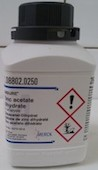
\includegraphics[]{../Bilder/20150504_141229.jpg}}
    \caption{Verwendete Chemikalien}
    \label{fig:Chemikalien}
\end{figure}

Die Sicherheitsdatenblätter sind in Anhang 4 - 8 zu finden.

\section{Verwendete Geräte}

Für die Probenvorbereitung und um die verschiedenen Lösungen herzustellen, werden diverse Laborgeräte verwendet. Diese sind in der folgenden Tabelle \ref{tab:Geräteliste} zusammengefasst.

\begin{table}[htbp]
    \centering
        \caption{Geräteliste}
        \begin{tabular}{l|C{0.25\linewidth}|c|c|c} 
            Anzahl & Gerät & Volumen in mL & Genauigkeit & Auslaufzeit\\
            \hline
            16 & Messkolben & 10 & A (+/- 0,040mL) & \\
            \hline
            8 & Messkolben & 50 & A (+/- 0,060mL) & \\
            \hline
            4 & Messkolben & 100 & A (+/- 0,100mL) & \\
            \hline
            4 & Vollpipetten & 1 & AS (+/- 0,006mL) & EX\\
            \hline
            2 & Vollpipetten & 2 & AS (+/- 0,010mL) & EX + 15s\\
            \hline
            1 & Vollpipetten & 5 & AS (+/- 0,015mL) & EX + 15s\\
            \hline
            1 & Vollpipetten & 10 & AS (+/- 0,02mL) & EX + 15s\\
            \hline
            1 & Vollpipetten & 20 & AS (+/- 0,03mL) & EX + 15s\\
            \hline
            1 & Messzylinder & 25 & & \\
            \hline
            diverse & Bechergläser & & & \\
            \hline
            1 & Wägeschiffchen & & & \\
            \hline
            1 & Analysenwaage Sartorius M-pact AX224 & max. 120g & d=0,1mg & 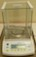
\includegraphics{../Bilder/20150504_140748.jpg}\\
            \hline
            1 & UV/VIS-Spektralphotometer Varian Cary® 50 & & & \\
            \hline
            1 & Präzisions-Küvette aus opt. Spezialglas & d=10mm & & \\
        \end{tabular}
    \label{tab:Geräteliste}
\end{table}


\section{Proben}

Es werden acht verschiedene Honige, ein Zuckerrübensirup und eine Invertzuckermischung vermessen. Die folgende Tabelle \ref{tab:Probenliste} zeigt die Probendetails.

\begin{table}[htbp]
    \centering
    \caption{Probenliste}
        \begin{tabular}{C{0.1\linewidth}|C{0.18\linewidth}|c|c|C{0.2\linewidth}|c} 
            Proben-nummer & Probe & Hersteller & Ablaufdatum & Herkunft & Lot-Nr.\\
            \hline
            1 & Flotte Biene Frühlings-blütenhonig & Langnese & 12.2016 & EU-Länder & LM41222\\
            \hline
            2 & Flotte Biene Gebirgs-blütenhonig & Langnese & 09.2016 & Nicht-EG-Länder & LI40946\\
            \hline
            3 & Sommer-blütenhonig & Vom Land & 06.2015 & EG- und Nicht-EG-Länder & L3442714\\
            \hline
            4 & Blütenhonig & Goldland & 03.2015 & EG- und Nicht-EG-Länder & LC40341\\
            \hline
            5 & Mexico & Biophar & 10.2016 & Mexiko & B582725\\
            \hline
            6 & Ägäis & Breitsamer & 07.2016 & Ägäis-Türkei & L4043131\\
            \hline
            7 & Waldhonig & Breitsamer & 10.2016 & Italien, Tschechien & L5644211\\
            \hline
            8 & Zuckerrüben-sirup & Grafschafter & 12.2017 & - & -\\
            \hline
            9 & Winterfutter & Imker B. Hahl & - & Walldorf, Deutschland & -\\
            \hline
            10 & Invertzucker & Pati-Versand.de & 09.2016 & - & 42090.58\\
        \end{tabular}
        \label{tab:Probenliste}
\end{table}

\begin{figure}[htbp]
    \centering
        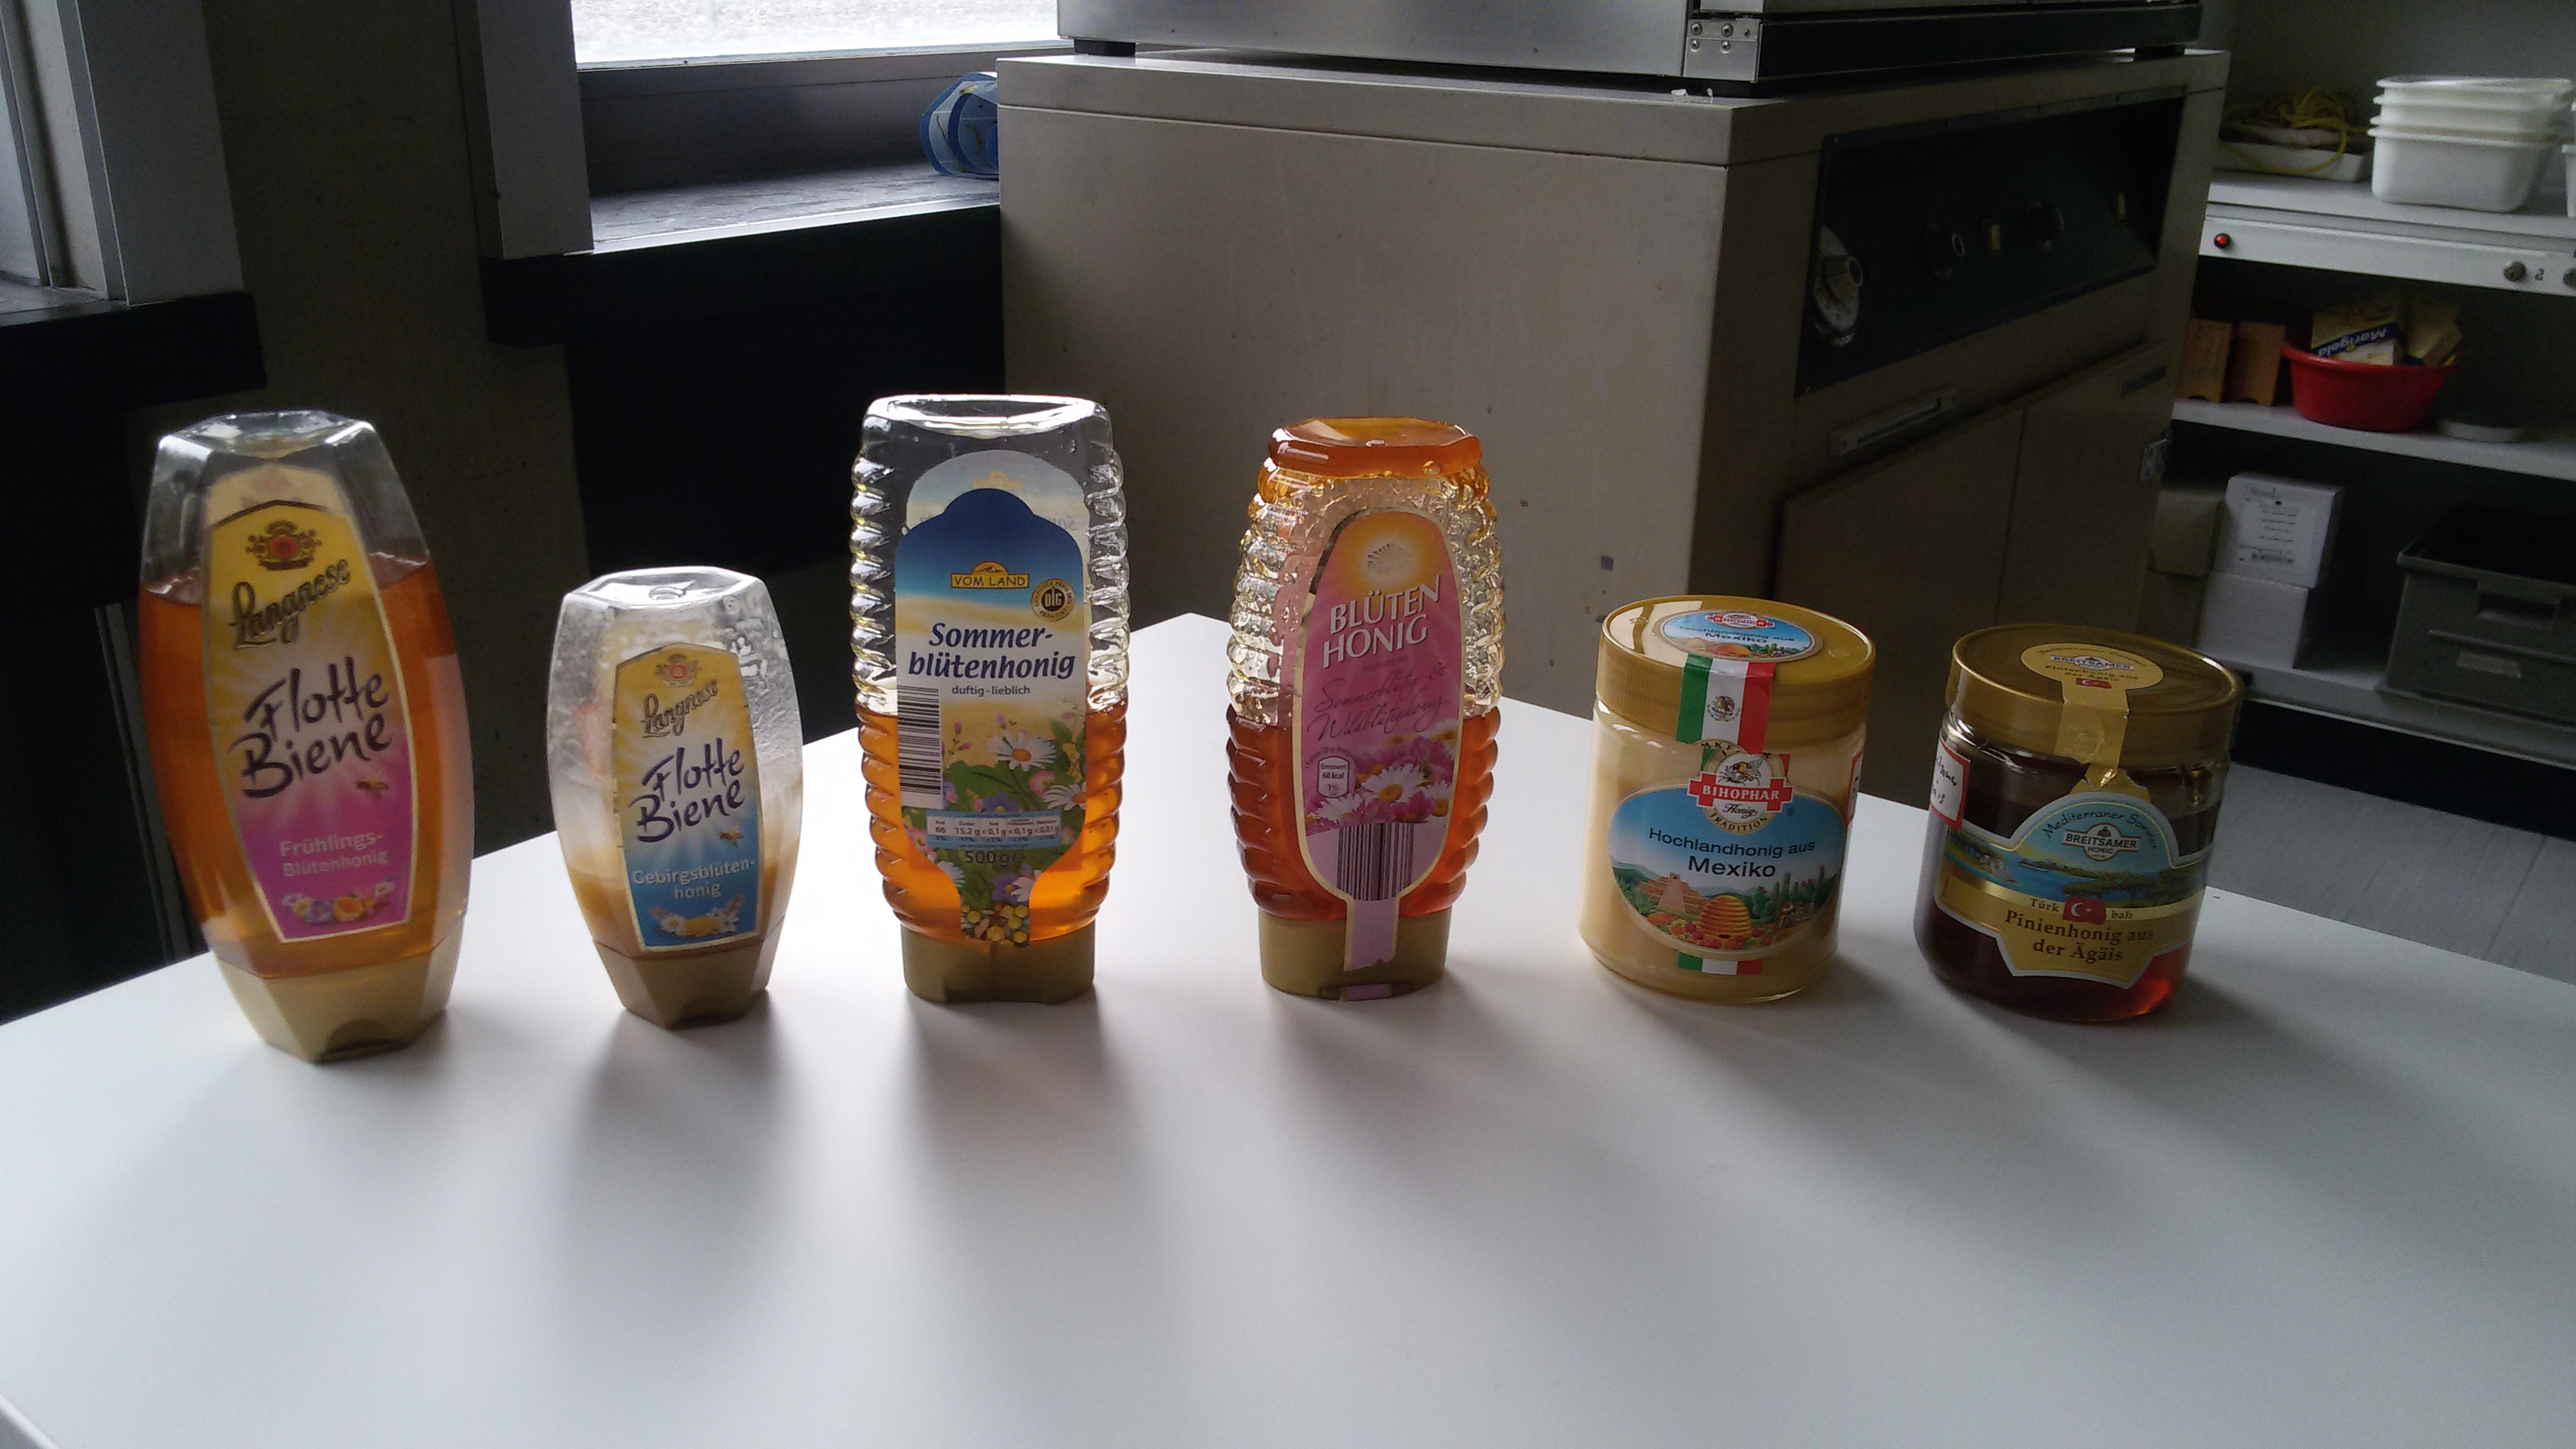
\includegraphics[width=1.00\textwidth]{../Bilder/20150416_183117.jpg}
    \caption{Übersicht der ersten sechs Honigproben}
    \label{fig:Honigproben}
\end{figure}


\section{Ansetzen der Reaktionslösungen}

Für die Probenaufbereitung werden zwei Carrez-Lösungen benötigt.\\ 
Für die Carrez-Lösung I wird am ersten Praktikumstag 15,1805g Kaliumhexacyanoferrat in einen 100mL Messkolben eingewogen, mit Wasser gelöst und bis zur Ringmarke aufgefüllt.\\ 
Die Carrez-Lösung II wurde zweimal angesetzt, da nach einer Woche Lagerung feste Partikel im Messkolben gefunden wurden. Am ersten Praktikumstag wurde für die Carrez-Lösung II 30,1485g Zinkacetat in einen 100mL Messkolben eingewogen, mit Wasser im Ultraschallbad gelöst und bis zur Ringmarke aufgefüllt. Da sich das Zinkacetat schlecht auflöste, wurde die Lösung beim zweiten Ansetzen am dritten Praktikumstag leicht erwärmt. Für die zweite Lösung wurde 30,0504g Zinkacetat eingewogen.\\ 
Die p-Toluidinlösung und die Barbitursäurelösung mussten nicht angesetzt werden, da sie in der benötigten Konzentration zur Verfügung standen. In der p-Toluidinlösung waren eine Woche nach Anbruch Feststoffpartikel enthalten.

\section{Ansetzen der Stammlösungen}

Für die Kalibrierreihe werden zwei Stammlösungen mit unterschiedlicher HMF-Konzentration angesetzt. Die Berechnung der benötigten Einwaagen befindet sich in Kapitel \ref{chap:Planung}.

\begin{figure}[htbp]
    \centering
        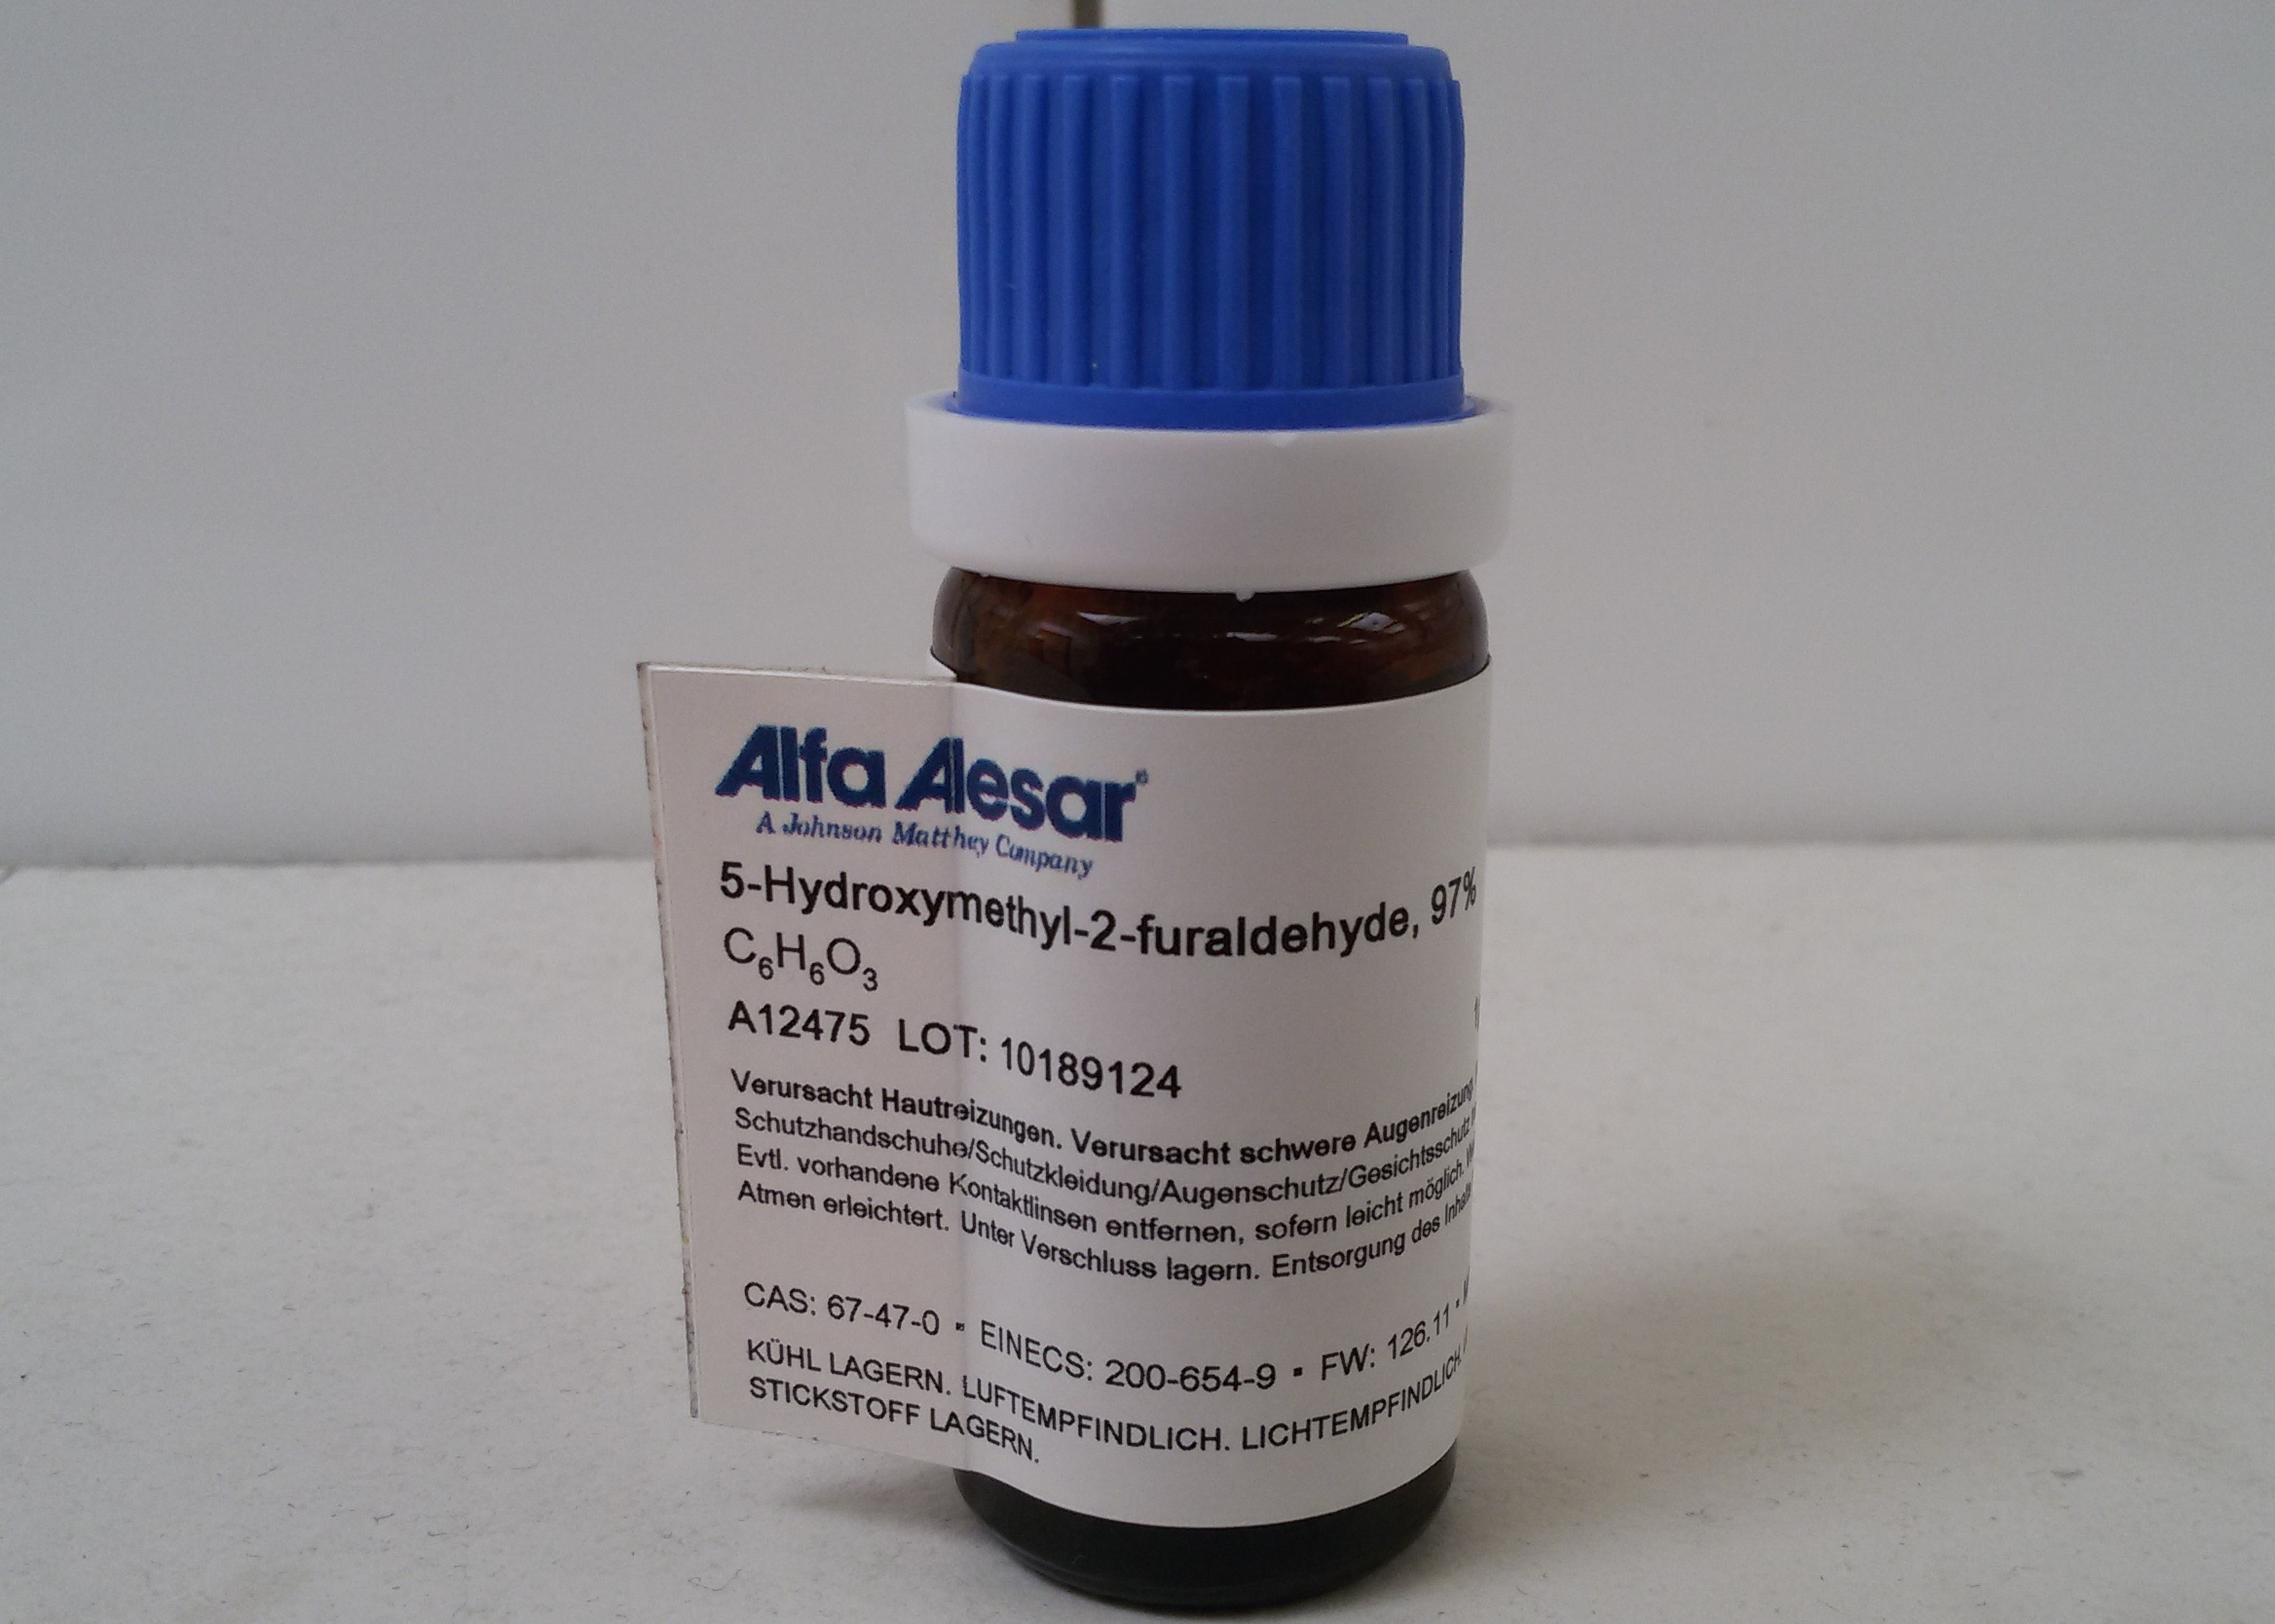
\includegraphics{../Bilder/20150504_140727.jpg}
    \caption{HMF-Reinsubstanz}
    \label{fig:HMF-Reinsubstanz}
\end{figure}
    
Die HMF-Reinsubstanz wird auf der Analysenwaage in einem Wägeschiffchen eingewogen, mit VE-Wasser in einen 10mL Messkolben überführt und bis zur Ringmarke aufgefüllt.\\
Einwaage SL1: 54,8mg\\
Einwaage SL2: 151,6mg\\
Aus den Einwaagen wird über die im Kapitel \ref{chap:Planung} verwendete Formel zur Konzentrationsberechnung die HMF-Konzentration der beiden Stammlösungen berechnet. Die Konzentration der Stammlösung 1 beträgt 5480mg/L und die Konzentration der Stammlösung 2 beträgt 15160mg/L.\\ 
Von beiden Stammlösungen wird je ein Milliliter in jeweils einen 100mL Messkolben überführt und mit VE-Wasser bis zur Ringmarke aufgefüllt. Somit ergibt sich für die Stammlösung 1.1 eine HMF-Konzentration von 54,8mg/L und für die Stammlösung 2.1 eine HMF-Konzentration von 151,6mg/L. 

    \section{Herstellung und Vermessung der Kalibrierlösungen}

    Für die Kalibrierlösungen werden aliquote Teile der beiden Stammlösungen 1.1 und 2.1 mit verschiedenen Vollpipetten in 50mL Messkolben abgefüllt und mit einigen Millilitern VE-Wasser vermischt. Die Berechnung der Volumina befindet sich im Kapitel \ref{chap:Planung}. Anschließend werden je 1mL Carrez-Lösung I und II mit einer Vollpipette hinzugefügt. Nach Durchmischen der Lösungen wird mit VE-Wasser bis zur Ringmarke aufgefüllt. Dabei fallen störende Matrixbestandteile als unlösliche Partikel aus.
    
    \begin{figure}[htbp]
      \centering
      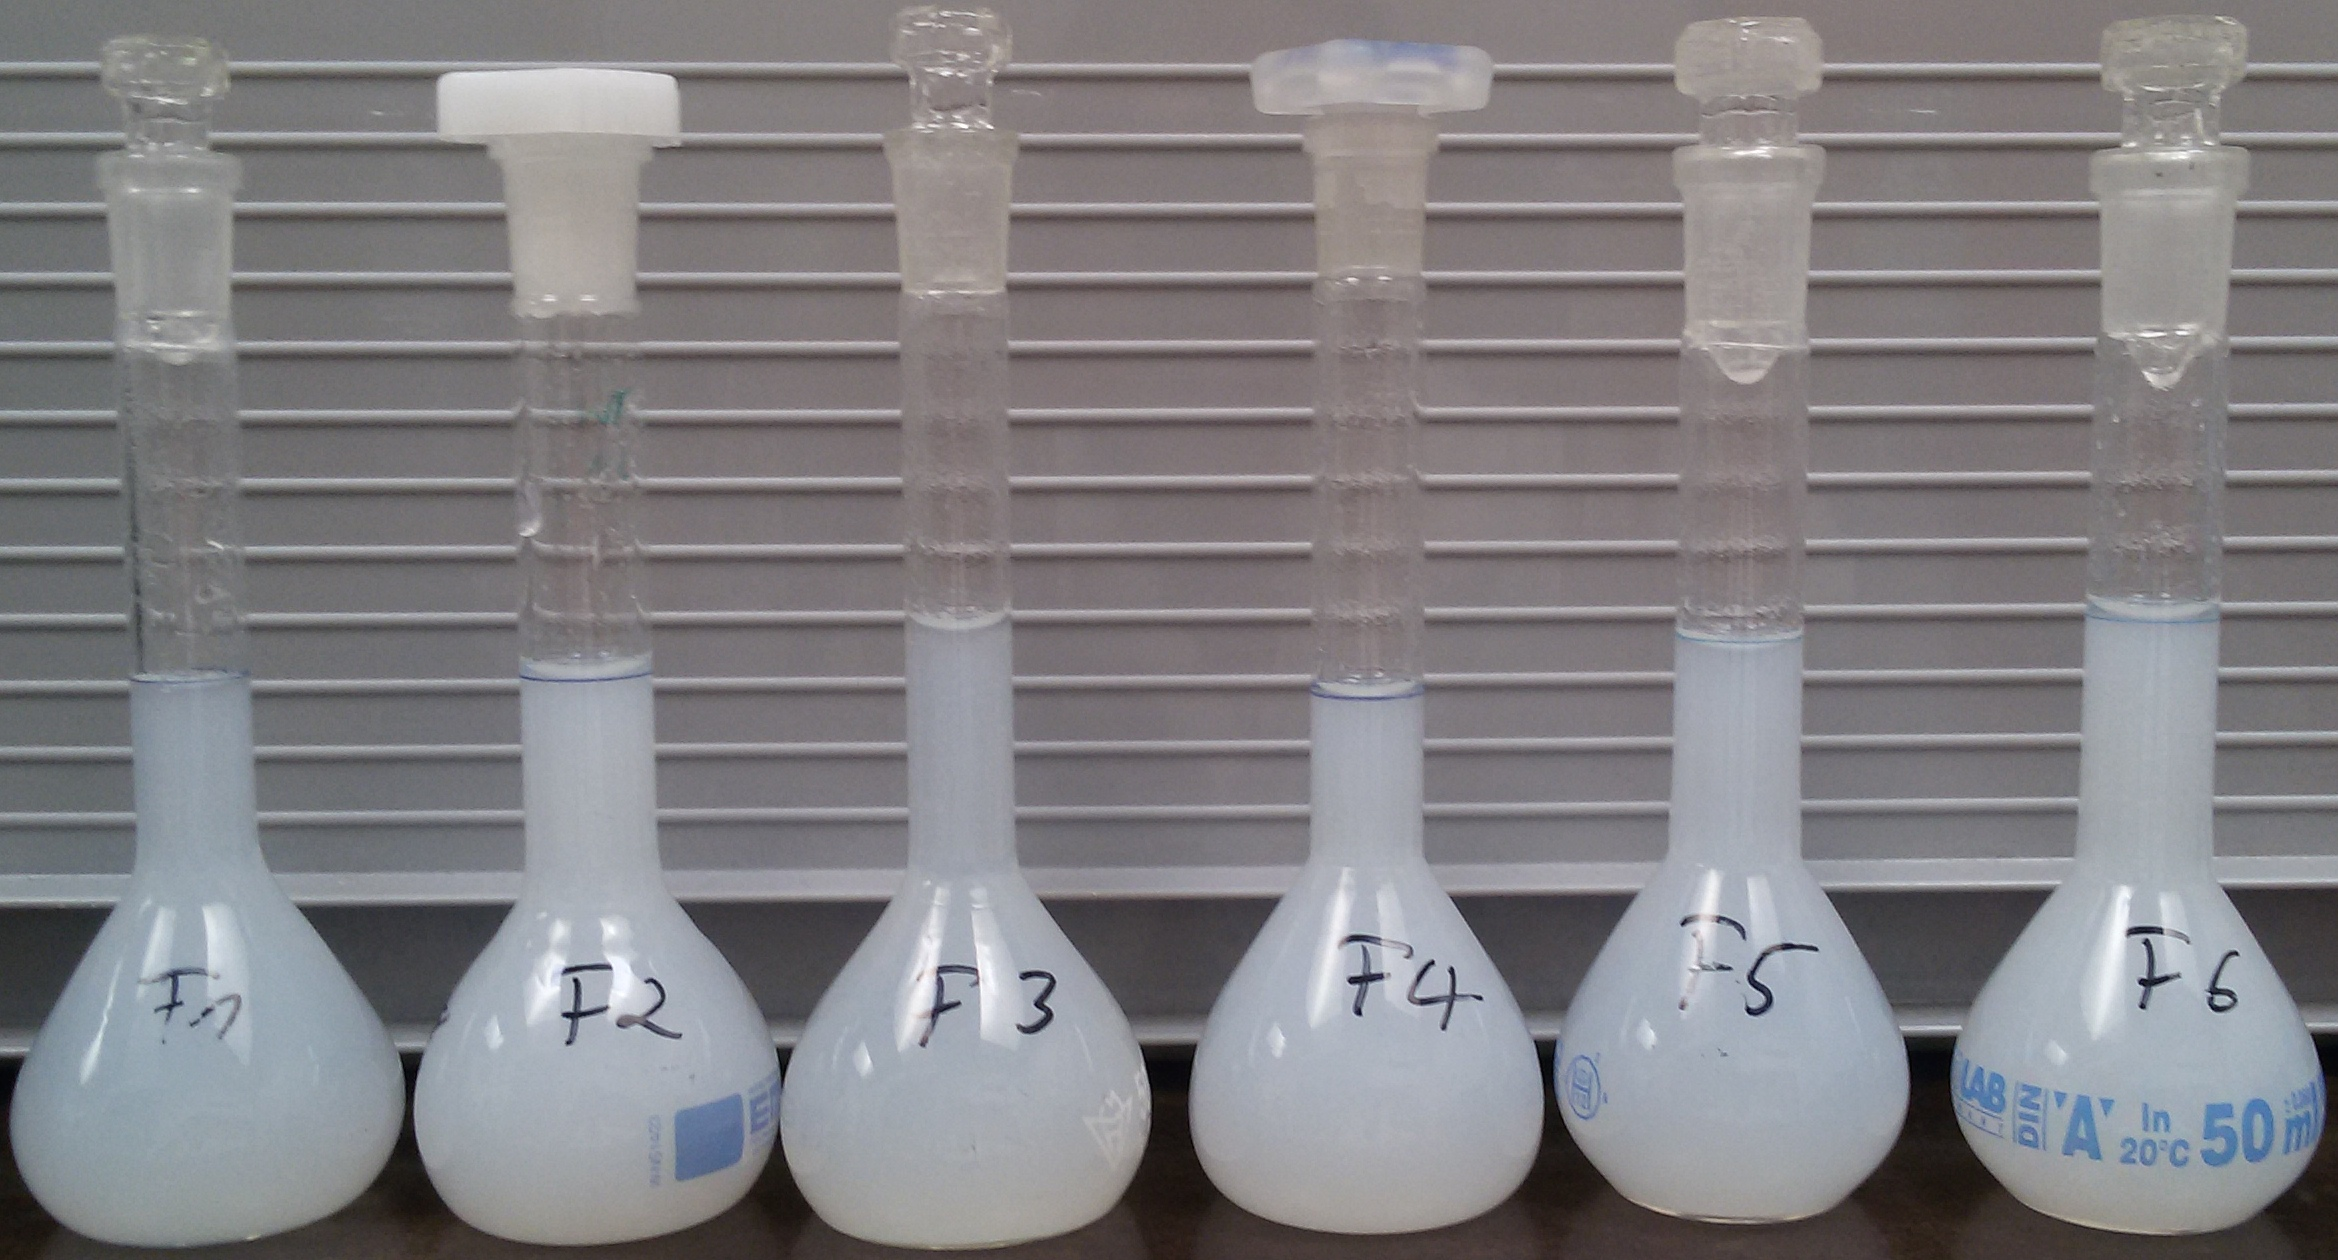
\includegraphics[width=1.00\textwidth]{../Bilder/20150424_155955.jpg}
      \caption{Kalibrierlösungen mit unlöslichen Partikeln}
      \label{fig:Partikel}
    \end{figure}
    
Die Lösungen werden über einen Faltenfilter filtriert, wobei die ersten 10mL Filtrat verworfen werden. Von dem restlichen Filtrat werden 2mL mit einer Vollpipette entnommen und in einen 10mL Messkolben überführt. In die Kolben werden außerdem jeweils 5mL p-Toluidinlösung und 1mL Barbitursäurelösung pipettiert. Von dem Filtrat der ersten Kalibrierlösung wird ebenfalls die Lösung für den Blindwert angesetzt. Hierbei werden 5mL p-Toluidinlösung zugegeben, aber anstelle der Barbitursäurelösung 1mL VE-Wasser zugesetzt. Zum Homogenisieren werden die Messkolben verschlossen und mehrmals invertiert. Da es sich bei der Farbreaktion um eine Zeitreaktion handelt, werden die Kalibrierlösungen und der Blindwert vor der Vermessung vier Minuten stehen gelassen. Danach müssen die Lösungen zügig vermessen werden, da der Farbkomplex nach dieser Zeit wieder zerfällt.\\
Mit der sechsten Kalibrierlösung wird die Wellenlänge des Absorptionsmaximums zwischen 200 und 800nm bestimmt. Der Ausdruck der Wellenlängenbestimmung ist in Anhang 1 zu finden.

\[
  \lambda_{max} = 550nm
\]

Dies entspricht der in der Literatur angegebenen Wellenlänge zur Vermessung des Farbkomplexes.~\cite{Winkler}\\
Die Kalibrierlösungen werden bei 550nm gegen den Blindwert vermessen und eine Kalibriergerade erstellt. Um Messfehler zu minimieren wird jede Kalibrierlösung dreimal gemessen.\\
In der nachfolgenden Tabelle \ref{tab:Kalibrierlösungen} sind die Kalibrierlösungen aufgelistet.

\begin{table}[htbp]
    \centering
    \caption{Kalibrierlösungen}
        \begin{tabular}{C{0.1\linewidth}|C{0.1\linewidth}|C{0.15\linewidth}|C{0.15\linewidth}|C{0.15\linewidth}|c} 
            Kalibrier-lösung & Stamm-lösung & Volumen Stamm-lösung\newline in mL & Massenkon-zentration berechnet\newline in mg/L & Massenanteil berechnet\newline in mg/kg & Extinktion\\
            \hline
            1 & 1.1 & 1 & 1,096 & 5,480 & 0,0400\\
            \hline
            2 & 1.2 & 1 & 3,032 & 15,16 & 0,1353\\
            \hline
            3 & 1.1 & 5 & 5,480 & 27,40 & 0,1687\\
            \hline
            4 & 1.1 & 10 & 10,96 & 54,80 & 0,3214\\
            \hline
            5 & 1.2 & 10 & 30,32 & 151,6 & 0,9453\\
            \hline
            6 & 1.2 & 20 & 60,64 & 303,2 & 1,8987\\
        \end{tabular}
        \label{tab:Kalibrierlösungen}
\end{table}

\begin{figure}[htbp]
    \centering
        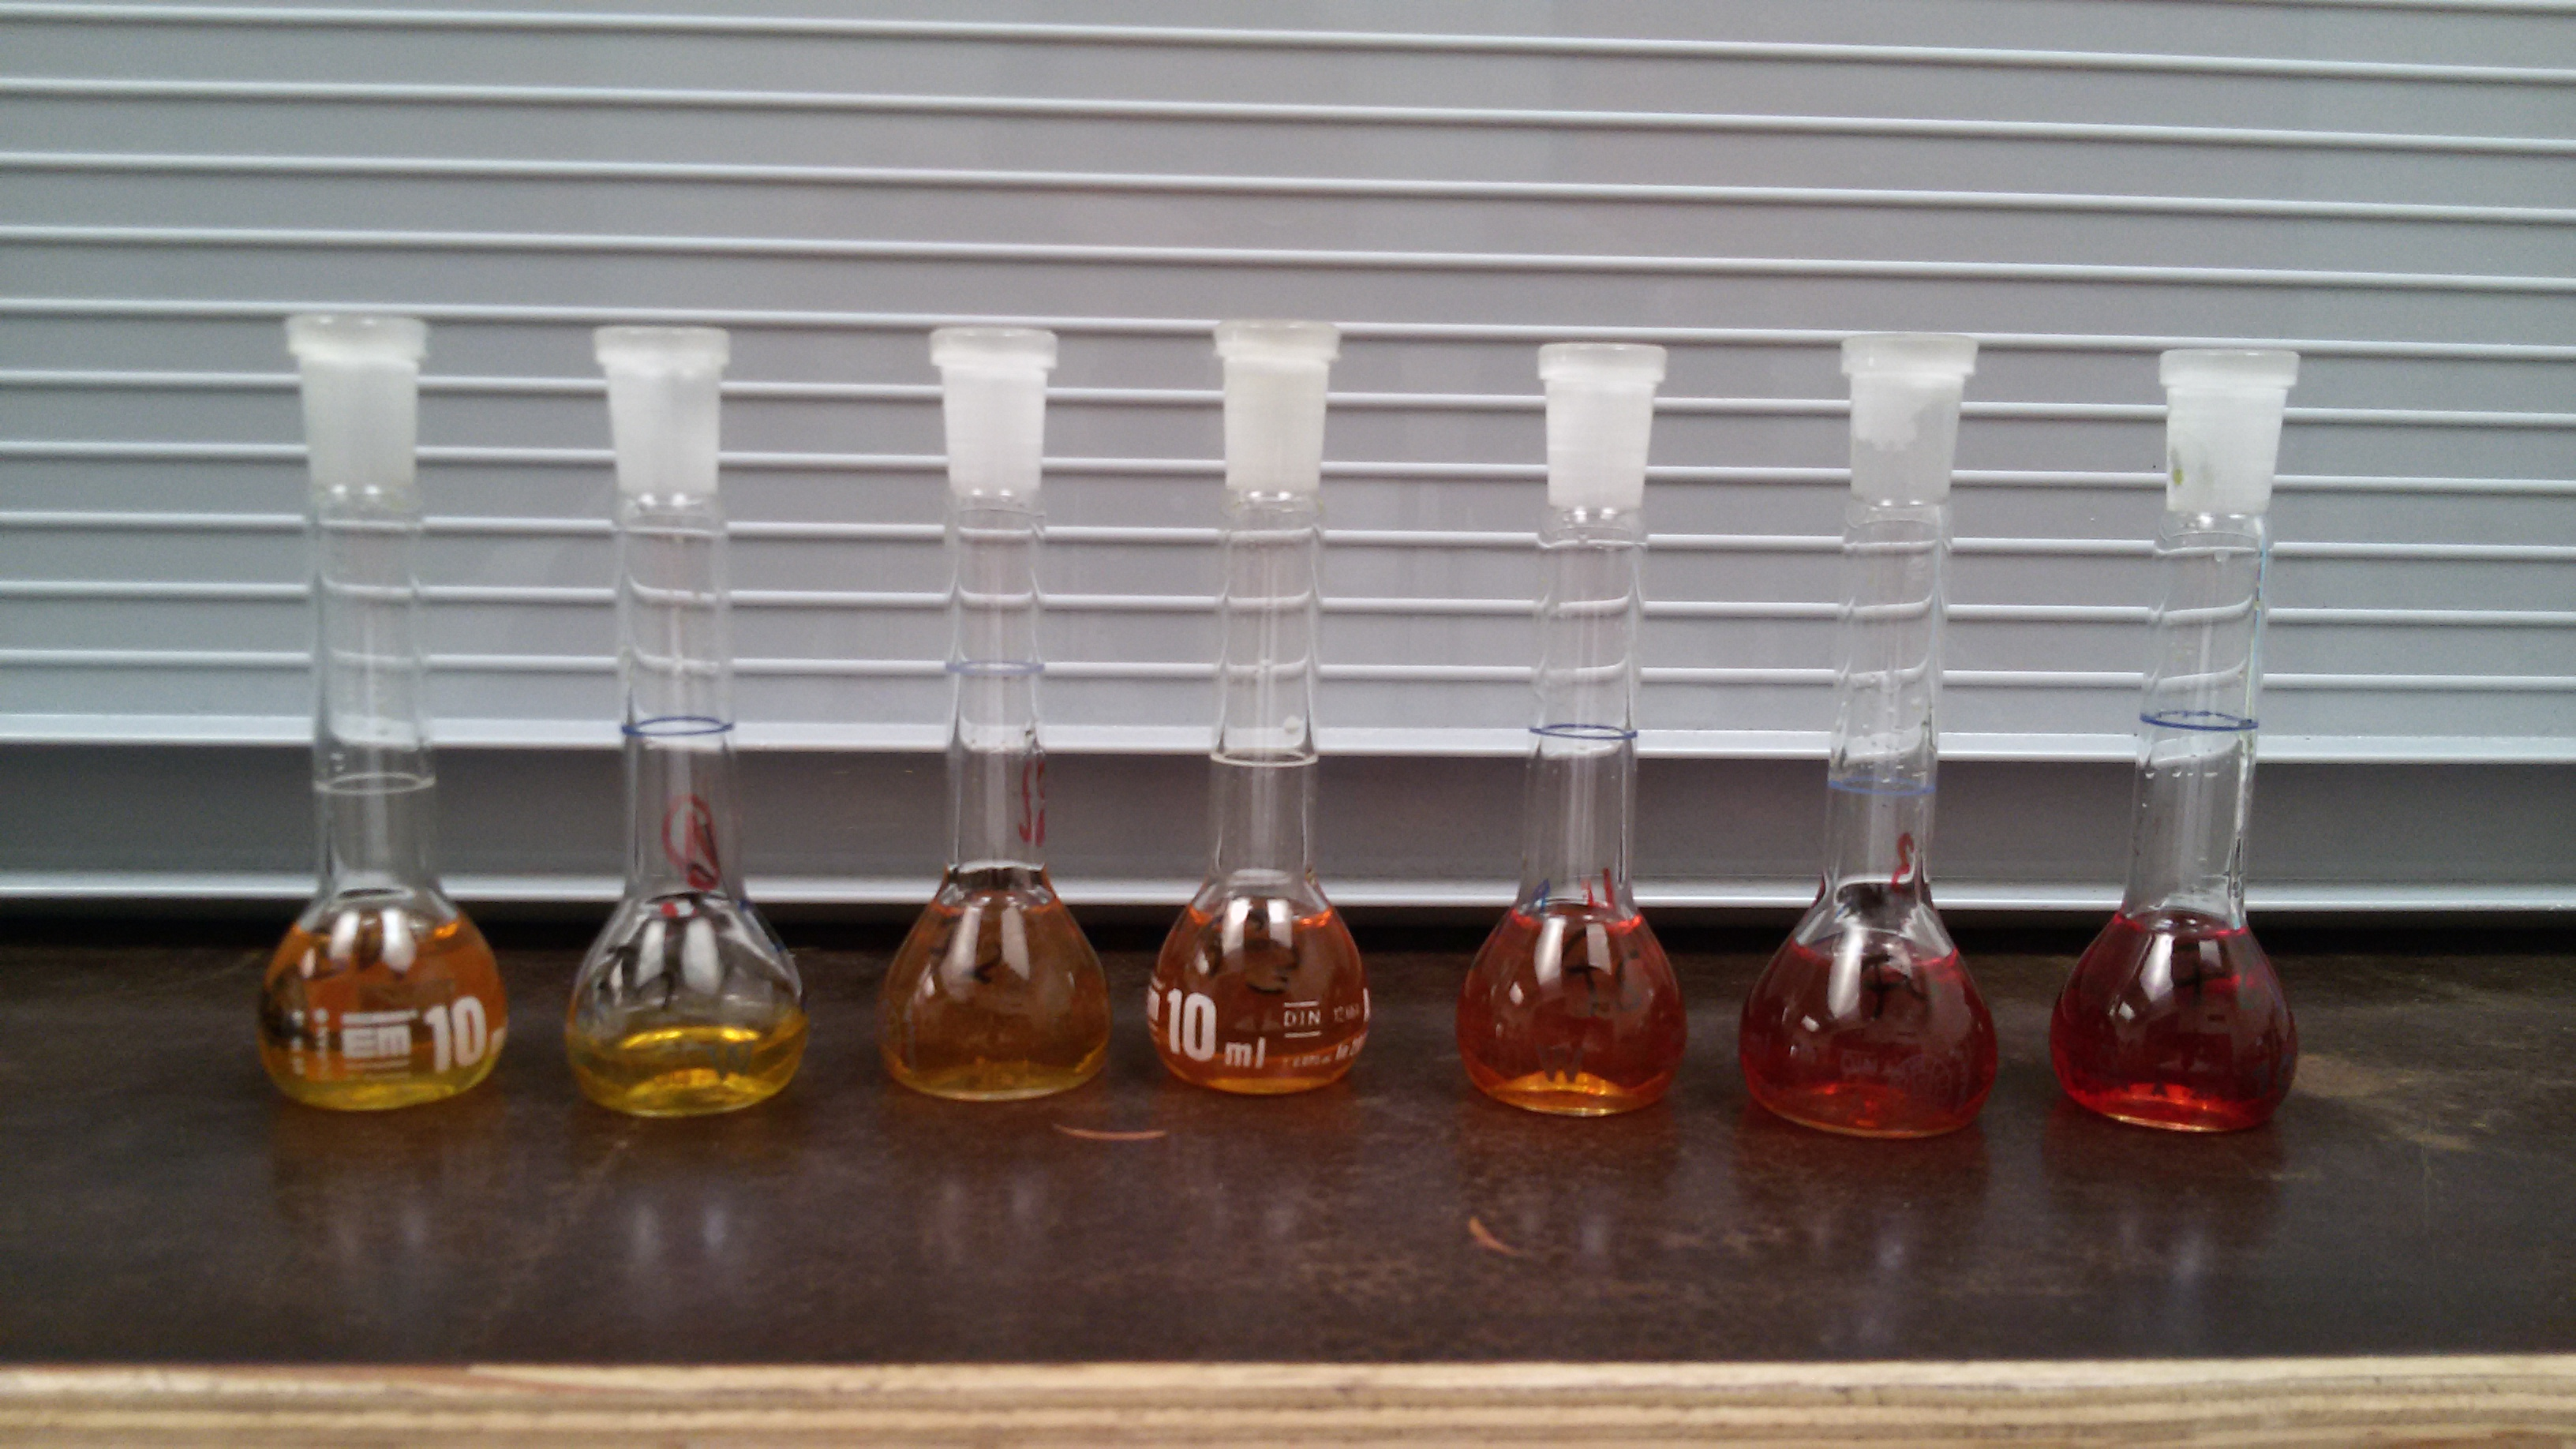
\includegraphics[width=1.00\textwidth]{../Bilder/20150424_172612.jpg}
    \caption{Kalibrierlösungen}
    \label{fig:Kalibrierlösungen}
\end{figure}


\section{Herstellung und Vermessung der Probelösungen}

Für die Probelösungen werden jeweils ca. 10g Probe in einen 50mL Messkolben eingewogen und in 20mL VE-Wasser gelöst. Die folgende Tabelle \ref{tab:Probeneinwaage} enthält die Lagertemperatur und die Einwaage der einzelnen Proben. 

\begin{table}[htbp]
    \centering
    \caption{Probeneinwaage}
        \begin{tabular}{c|c|c} 
            Probennummer & Lagertemperatur in $^\circ$C & Einwaage in g\\
            \hline
            1 & 25 & 10,2926\\
            \hline
            1 & 60 & 11,0590\\
            \hline
            2 & 25 & 10,2548\\
            \hline
            2 & 60 & 10,0891\\
            \hline
            3 & 25 & 11,3998\\
            \hline
            3 & 60 & 10,2277\\
            \hline
            4 & 25 & 9,9125\\
            \hline
            4 & 60 & 10,0411\\
            \hline
            5 & 25 & 10,0203\\
            \hline
            5 & 60 & 10,2194\\
            \hline
            6 & 25 & 10,0776\\
            \hline
            6 & 60 & 10,0968\\
            \hline
            7 & 25 & 10,4448\\
            \hline
            8 & 25 & 10,4160\\
            \hline
            9 & 25 & 10,1488\\
            \hline
            10 & 25 & 9,9153\\
        \end{tabular}
    \label{tab:Probeneinwaage}
\end{table}

Jeder Probelösung werden je 1mL Carrez-Lösung I und II zugesetzt und die Messkolben nach dem Homogenisieren mit VE-Wasser bis zur Ringmarke aufgefüllt. Die ausgefallenen Partikel werden über Faltenfilter abfiltriert.

\begin{figure}[htbp]
    \centering
        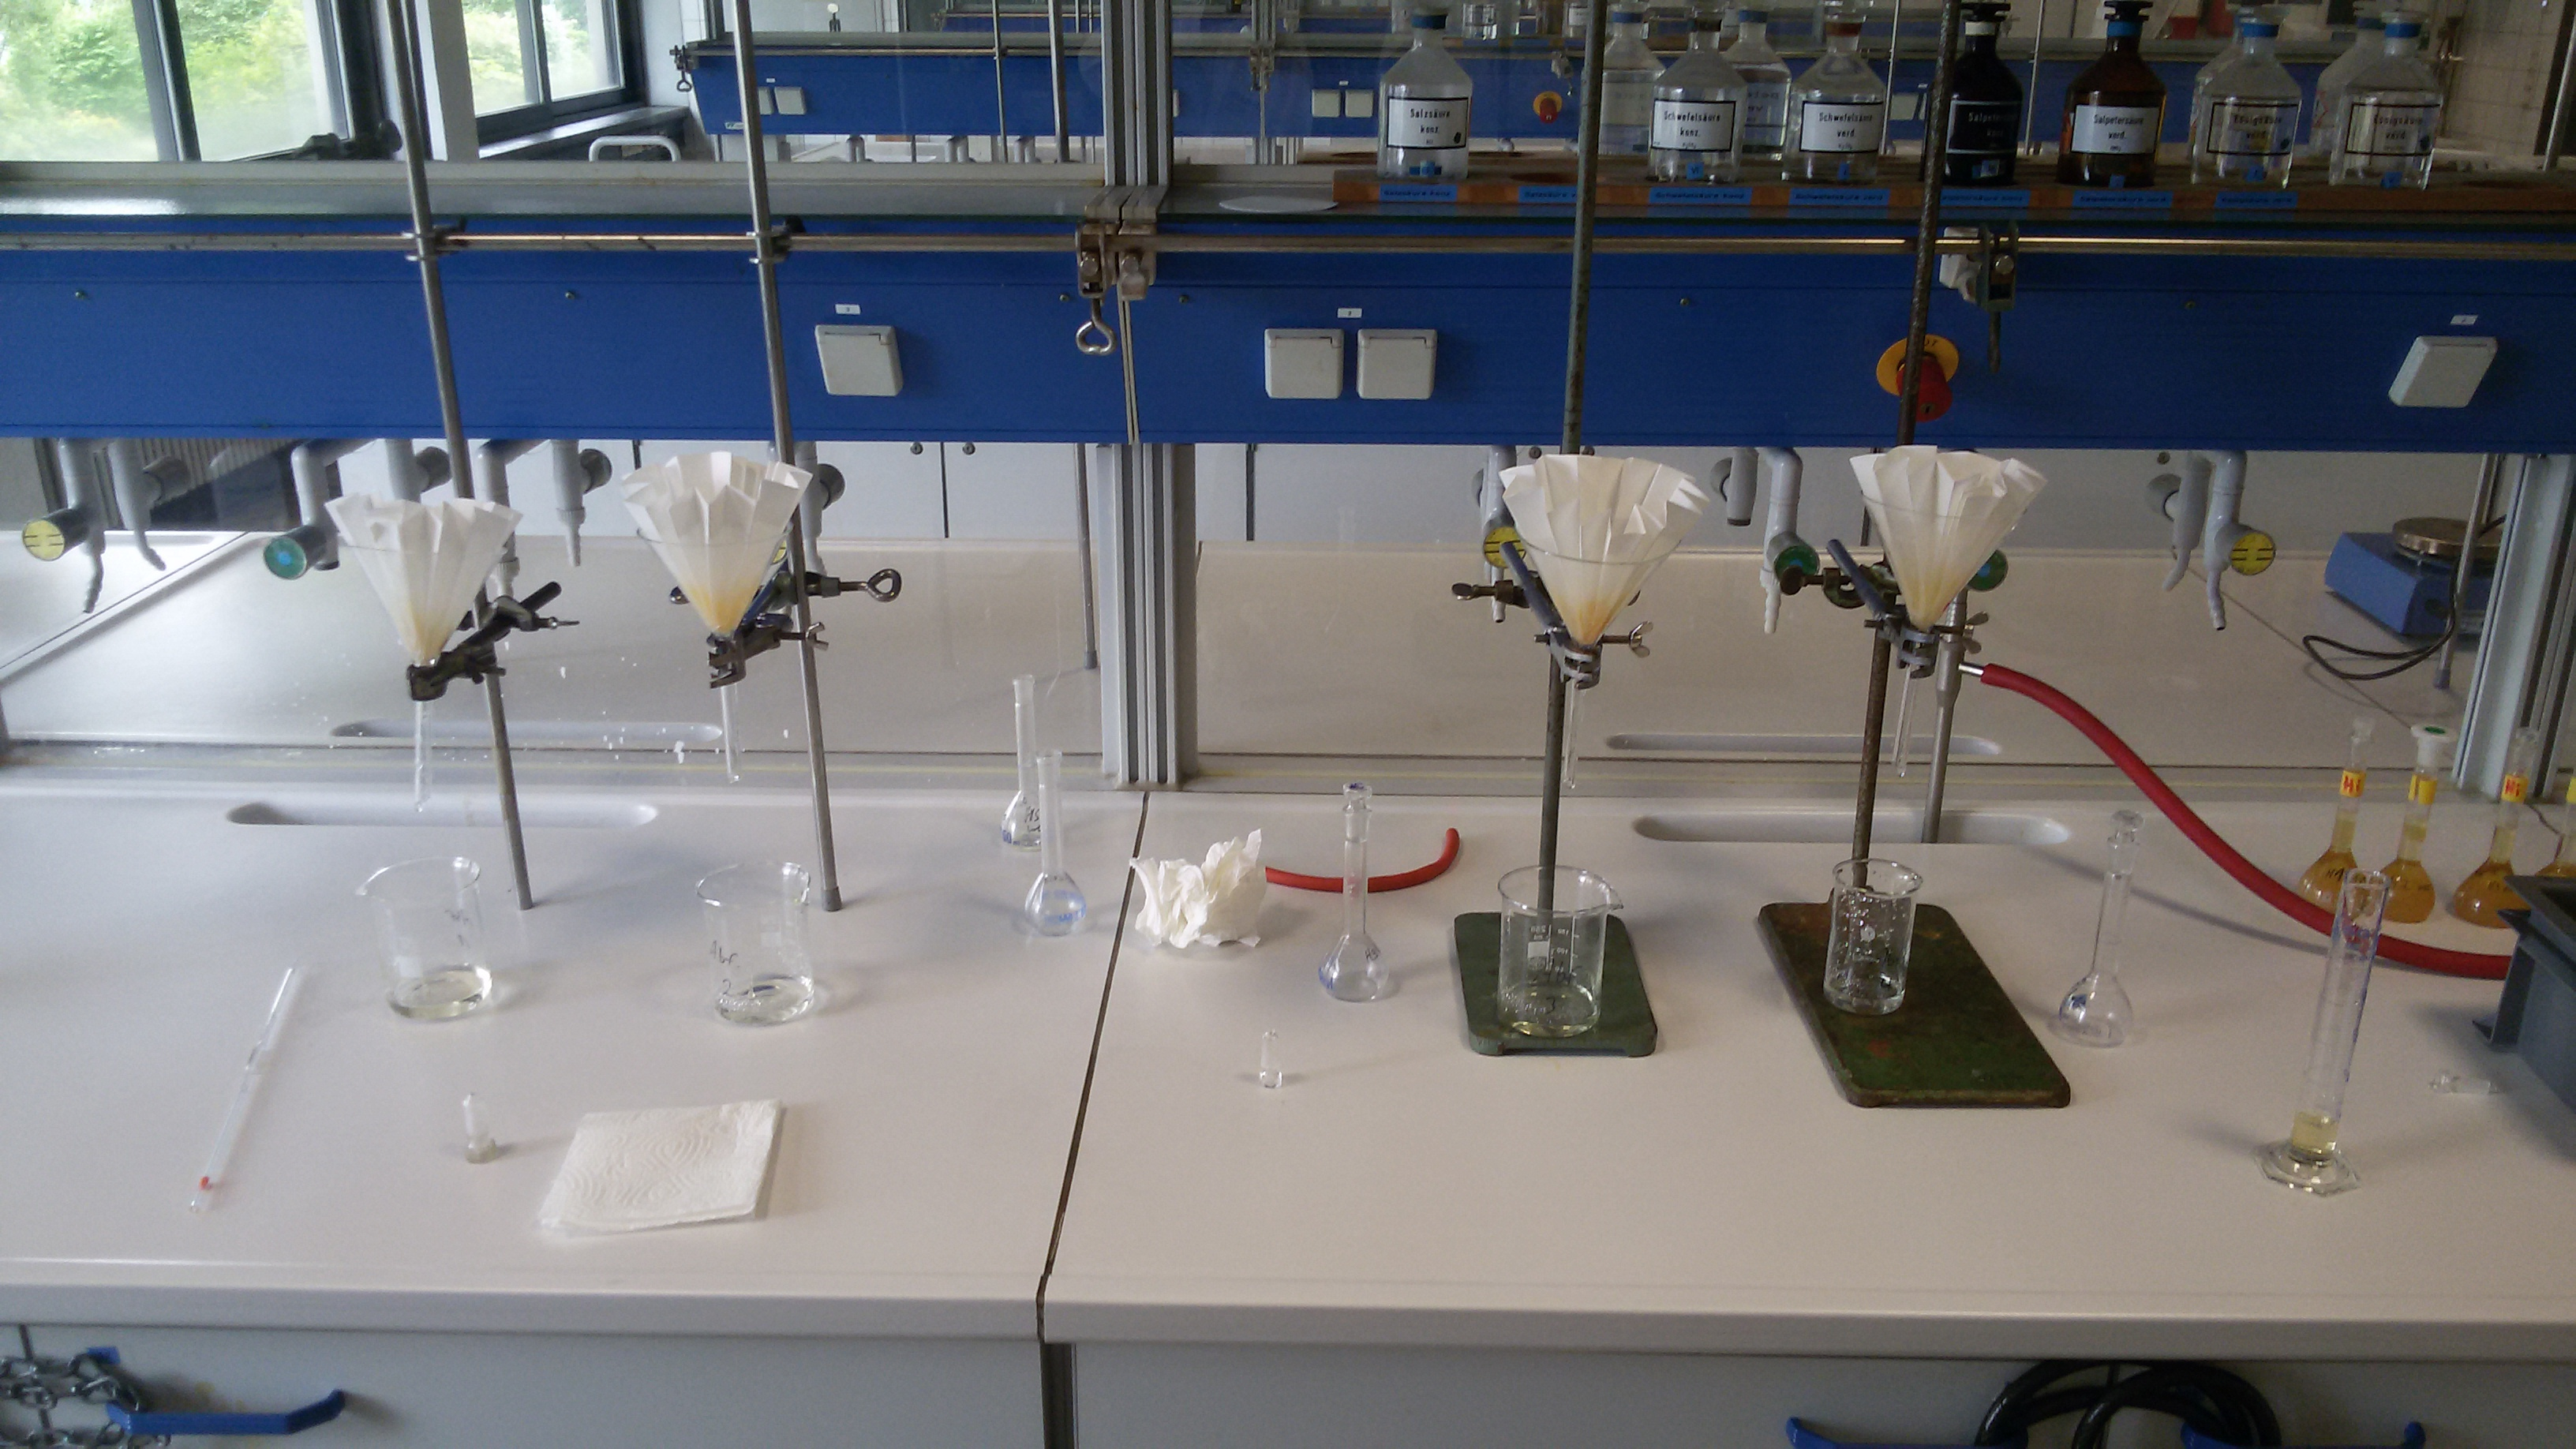
\includegraphics[width=1.00\textwidth]{../Bilder/20150427_131648.jpg}
    \caption{Filtration der Proben}
    \label{fig:Filtration}
\end{figure}

Dabei werden die ersten 10mL des Filtrats verworfen. Von dem Filtrat werden mit einer Vollpipette jeweils zweimal 2mL entnommen und in zwei 10mL Messkolben überführt. In einem Messkolben wird der Blindwert angesetzt, im anderen die zu vermessende Probe. In beide Messkolben werden je 5mL p-Toluidinlösung hinzugefügt. Mit einer 1mL Vollpipette wird dem Blindwert 1mL VE-Wasser zugegeben und der Probelösung 1mL Barbitursäurelösung. Beide Messkolben bleiben nach dem Homogenisieren für vier Minuten stehen. Die Messung der Probe erfolgt danach bei 550nm gegen den jeweiligen Blindwert. Die Proben werden jeweils dreimal vermessen um Messfehler möglichst gering zu halten.
\begin{figure}[htbp]
    \centering
        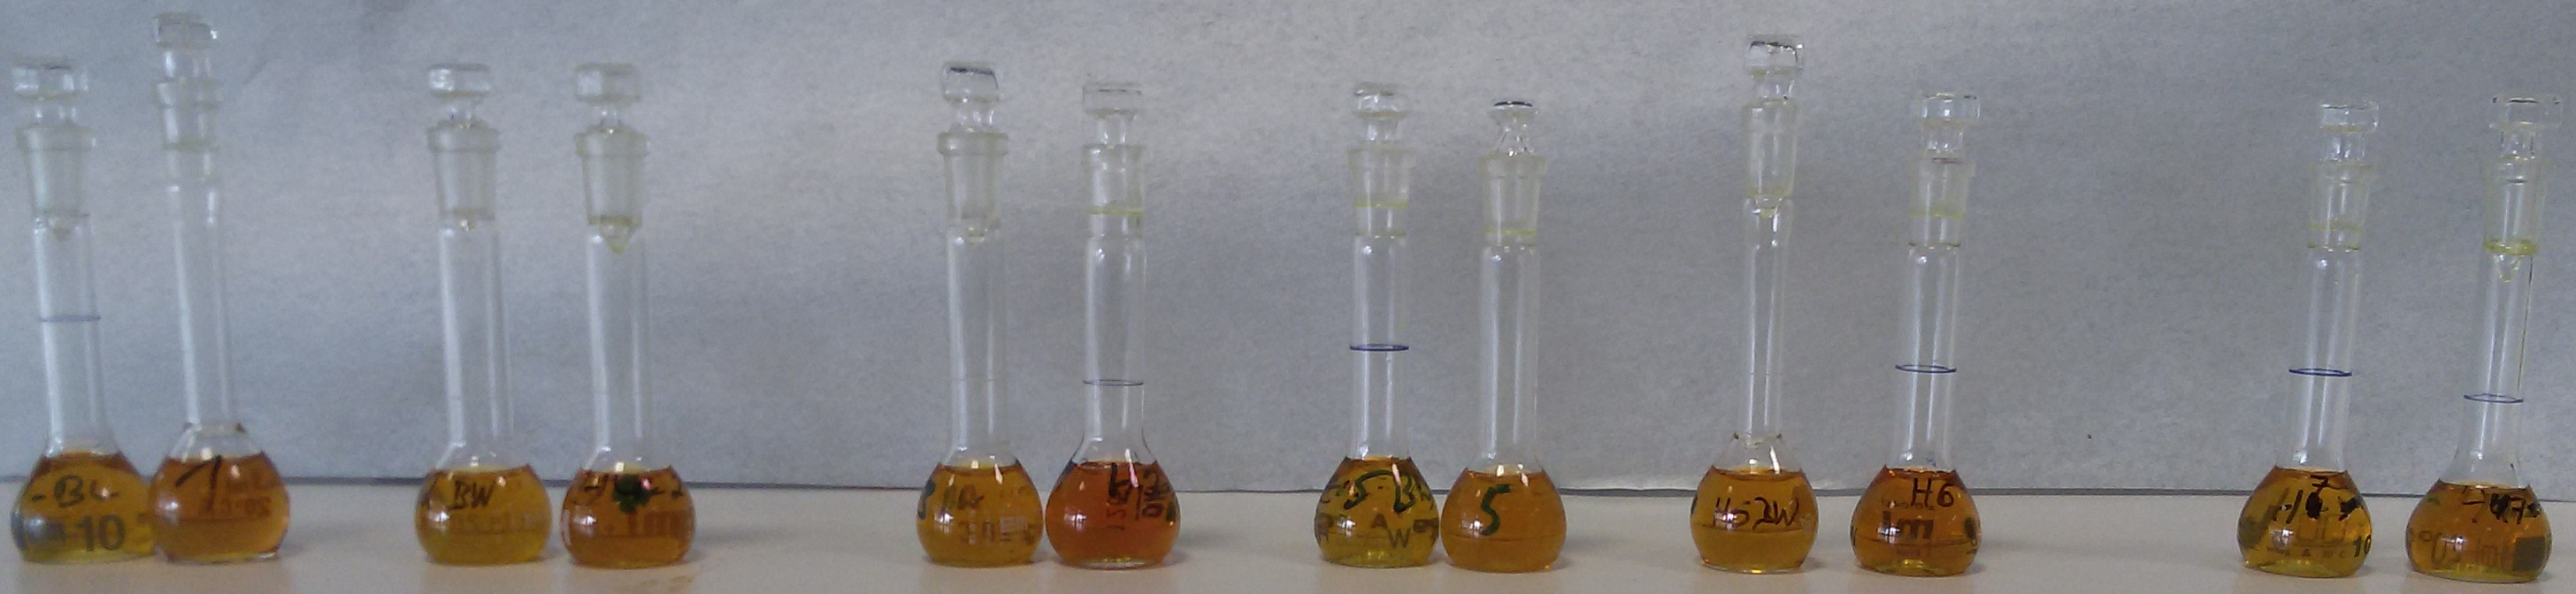
\includegraphics[width=1.00\textwidth]{../Bilder/20150427_140221(0).jpg}
    \caption{Probenauswahl mit Blindwerten}
    \label{fig:Probenauswahl}
\end{figure}

\newpage
\section{Mehrfachbestimmung und Aufstockung einer Probe}

Für eine Mehrfachbestimmung wird die Honigprobe 3 am zweiten Praktikumstag einmal und am dritten Praktikumstag sechsmal eingewogen, wie oben beschrieben mit Reaktionslösungen versetzt und anschließend vermessen. Außerdem werden zwei zusätzliche Einwaagen der Honigprobe 3 einmal mit 10mL der Stammlösung 1.1 und einmal mit 5mL der Stammlösung 2.1 versetzt und so der HMF-Gehalt aufgestockt. Diese beiden Proben werden ebenfalls wie oben beschrieben behandelt und vermessen. Die Einwaagen sind in folgender Tabelle \ref{tab:Probeneinwaage Mehrfachbestimmung + Aufstockungen} aufgeführt:
\begin{table}[htbp]
    \centering
    \caption{Probeneinwaage Mehrfachbestimmung + Aufstockungen}
        \begin{tabular}{c|c|c} 
            Probennummer & Lagertemperatur in $^\circ$C & Einwaage in g\\
            \hline
            3.1 & 25 & 10,323\\
            \hline
            3.2 & 25 & 10,358\\
            \hline
            3.3 & 25 & 10,199\\
            \hline
            3.4 & 25 & 10,835\\
            \hline
            3.5 & 25 & 10,414\\
            \hline
            3.6 & 25 & 10,286\\
            \hline
            3.7 Aufst.1 & 25 & 10,483\\
            \hline
            3.8 Aufst.2 & 25 & 10,365\\
        \end{tabular}
    \label{tab:Probeneinwaage Mehrfachbestimmung + Aufstockungen}
\end{table}

\chapter{Auswertung}
Der HMF-Gehalt der Proben wird mit zwei Methoden bestimmt. Diese werden im folgenden Abschnitt vorgestellt, angewandt und miteinander verglichen. Außerdem wird die Genauigkeit der beiden Methoden über die Wiederfindungsrate überprüft.
\section{Kalibrierung}
Zur Bestimmung von HMF wird eine Kalibrierung durchgeführt. Um die Linearität des Messsignals bei verschiedenen Konzentrationen zu gewährleisten müssen mehrer Kalibrierlösungen vermessen werden. Da ein von 5 bis 300mg/kg großer Bereich abgedeckt werden soll fiel die Entscheidung auf sechs Messpunkte. Die Konzentrationen der Kalibrierstandard sind in folgender Tabelle aufgetragen:

\begin{table}[htbp]
	\centering
		\begin{tabular}{p{0.30\linewidth}|p{0.25\linewidth}|p{0.25\linewidth}|p{0.2\linewidth}}
			Standard & Extinktion & Konzentration / [mg/L] &  Massenanteil / [mg/kg]\\
			\hline
			Std 1 & 0,0400 & 1,004 & 5\\
			\hline
			Std 2 & 0,1353 & 3,032 & 15\\
			\hline
			Std 3 & 0,1687 & 5,020 & 25\\
			\hline
			Std 4 & 0,3214 & 10,040 & 50\\
			\hline
			Std 5 & 0,9453 & 30,320 & 152\\
			\hline
			Std 6 & 1,8987 & 60,640 & 303
		\end{tabular}
	\caption{Kalibrierungen}
	\label{tab:Kalibrierungen}
\end{table}

Die abgegebenen Gehalte und Konzentrationen beziehen sich auf eine theoretische Probeneinwaage von 10,0g Honig.\\
Trägt man nun die Kalibrierpunkte in einem Diagramm ein ergibt sich eine Gerade mit der Funktion $y=0,0309*x+0,0175$ bei einem Bestimmtheitsmaß von 0,9997.
%Diagramm mit Kalibriergeraden hier einfügen

\section{Quantifizierung mittels Kalibriergerade}
Die durch die Kalibrierung ermittelte Funktion wird zur Bestimmung des Analytgehalts verwendet.
	\[y=m*x+b\]
	\[y=0,0309*x+0,0175\]
	\[x=\frac{ y-0,0175 }{ 0,0309 }\]
Beispielrechnung zu Probe 3 (warm):
	\[x=\frac{ 1,9812-0,0175 }{ 0,0309 }\]
	\[x=63,55mg/L\]
Die Massenkonzentration muss nun noch in den Massenanteil umgerechnet werden.
	\[w[mg/kg]=\frac{ \beta*V }{ 1L * m }*1000000\]
	\[w[mg/kg]=\frac{ 0,06355g/L*0,05L }{ 1L * 10,041g }*1000000\]
	\[w[mg/kg]=316mg/kg\]

	
\section{Quantifizierung mittels Festfaktor}
In der Analysevorschrift zur Bestimmung von HMF in Honig ist folgende Formel angegeben:
	\[HMF[mg/kg]=\frac{ E * 1920 }{ m }\]
Hierbei steht E für die Extinktion, m für die Probenmasse und der Festfaktor 1920 setzt sich zusammen aus dem molaren Extinktionskoeffizienten und der Verdünnung und Umrechnung in die gewünschte Einheit mg/kg.
	\[Faktor=\frac{ M(HMF)*V }{ \epsilon }*1000000\]
	
	\[1920=\frac{ 126g/mol * 0,05L }{ 3,28125L/mol }*1000000\]
Beispielrechnung zu Probe 3 (warm):
	\[HMF[mg/kg]=\frac{ 1,9812 * 1920 }{ 10,041g }\]
	\[HMF[mg/kg]=379mg/kg\]
\section{Ergebnisse der analysierten Proben}
Alle Proben wurden mit den beiden zur Verfügung stehenden Methoden quantifiziert und in einer Tabelle aufgetragen.

\begin{table}[htbp]
	\centering
		\begin{tabular}{p{0.30\linewidth}|p{0.17\linewidth}|p{0.25\linewidth}|p{0.25\linewidth}} 
			Probenbezeichnung & Extinktion & Gehalt HMF über Kalibrierung \ [mg/kg] &  Gehalt HMF über Festfaktor \ [mg/kg]\\
			\hline
			1 Flotte Biene Frühlingsblütenhonig (kalt) & 0,016 & <5 & <5\\
			\hline
			1 Flotte Biene Frühlingsblütenhonig (warm) & 1,6041 & 256 & 307\\
			\hline
			2 Flotte Biene Gebirgsblütenhonig (kalt) & 0,0102 & <5 & <5\\
			\hline
			2 Flotte Biene Gebirgsblütenhonig (warm) & 1,3184 & 210 & 252\\
			\hline
			3 Sommerblütenhonig (kalt) & 0,1500 & 20 & 27\\
			\hline
			3 Sommerblütenhonig (warm) & 1,9812 & 316 & 379\\
			\hline
			4 Blütenhonig (kalt) & 0,0621 & 7 & 12\\
			\hline
			4 Blütenhonig (warm) & 1,5500 & 245 & 294\\
			\hline
			5 Mexico (kalt) & 0,0639 & 8 & 12\\
			\hline
			5 Mexico (warm) & 1,2237 & 194 & 234\\
			\hline
			6 Ägäis (kalt) & 0,0871 & 11 & 16\\
			\hline
			6 Ägäis (warm) & 1,1639 & 185 & 223\\
			\hline
			7 Waldhonig & 0,0362 & <5 & 7\\
			\hline
			8 Zuckerrübensirup & n.B. & n.B. & n.B.\\
			\hline
			9 Winterfutter & 0,0255 & <5 & 5\\
			\hline
			10 Invertzucker & 1,541 & 249 & 298\\

		\end{tabular}
	\caption{Messergebnisse}
	\label{tab:Messergebnisse}
\end{table}

\section{Wiederfindungsrate}
Da zur Bestimmung des HMF-Gehalts nur ideale Kalibrierlösungen bzw. der angegebene Festfaktor verwendet wurden, muss der Einfluss der Probenmatrix auf das Analysenergebnis ermittelt werden. Hierzu wird die Wiederfindungsrate anhand einer Aufstockung ermittelt. Die Wiederfindungsrate (WFR) ist der Quotient aus dem Istwert und dem Sollwert der Probe. Zur Berechnung der Wiederfindung wird die folgende Formel verwendet:
	\[WFR=\frac{ Gefundener Gehalt + Istwert }{ Gefundener Gehalt + Sollwert } *100 \]
Als Gefundener Gehalt wird der Mittelwert aus der Sechsfachbestimmung der Probe 3 verwendet.
	\[x(Mittelwert)=\frac{ x1+x2...xn }{ n } \]
Die Berechnung des Mittelwertes nach dem in der Vorschrift angegeben  Festfaktor:
	\[28mg/kg=\frac{ 29mg/kg+31mg/kg+25mg/kg+25mg/kg+31mg/kg+28mg/kg }{ 6 } \]
Die Berechnung des Mittelwertes nach der erstellten Kalibriergerade:
	\[21mg/kg=\frac{ 22mg/kg+23mg/kg+18mg/kg+19mg/kg+23mg/kg+21mg/kg }{ 6 } \]
Nach dem gemittelten Gehalt muss der aufgestockte Anteil an Analyt berechnet werden. In eine Aufstockung wurden 10ml der Stammlösung 1.1 zugegeben. Das entspricht einer Masse von 0,502 mg. Bezogen auf die Probeneinwaage von 10,483g ergibt sich ein theoretischer Massenanteil von:  
	\[w=\frac{ m(Analyt) }{ m(Gesamt) } \]
	\[47,9mg/kg=\frac{ 0,502mg }{ 0,010483kg } \]
In einer zweiten Aufstockung wurden 5ml Stammlösung 2.1 zugegeben, was einer Masse von 0,758mg entspricht. Auch hier wird mit der Einwaage von 10,365g der theoretische Massenanteil berechnet:
	\[73,1mg/kg=\frac{ 0,758mg }{ 0,010365kg } \]
Mit den Mittelwerten und den theoretischen kann die Wiederfindungsrate berechnet werden.\\
Zuerst die erste Aufstockung anhand des Festfaktors:
	\[92,3=\frac{ 28mg/kg + 47,9mg/kg }{ 82mg/kg } *100 \]
Und nach der Kalibriergeraden:
	\[104,4=\frac{ 21mg/kg + 47,9mg/kg }{ 66mg/kg } *100 \]
Anhand der beiden Wiederfindungsraten kann man darauf schließen, dass die Quantifizierung mit der Kalibriergeraden richtigere Werte liefert. Zur Kontrolle werden beide Berechnungen noch einmal mit der zweiten Aufstockung durchgeführt.\\
Bestimmung der zweiten Aufstockung nach Festfaktor:
	\[95,4=\frac{ 28mg/kg + 73,1mg/kg }{ 106mg/kg } *100 \]
Bestimmung der zweiten Aufstockung nach Kalibriergeraden:
	\[108,2=\frac{ 21mg/kg + 73,1mg/kg }{ 87mg/kg } *100 \]
Beide Wiederfindungsraten sind nahe 100 \% jedoch findet man mit der Kalibriergeraden tendenziell leicht erhöhte Gehalte an HMF wieder, während man in den Proben weniger HMF findet. Es ist auch bemerkenswert wie gut der angegebene Festfaktor zur Gehaltsbestimmung geeignet ist obwohl bei seiner Verwendung in keinster Weise kalibriert wird und das verwendete Messgerät damit völlig ignoriert wird. Auch bei der Richtigkeit der Ergebnisse sind beide Methoden vergleichbar.
	
\section{Standardaddition}
Da die Probe 3 zweimal mit unterschiedlichen Mengen an HMF aufgestockt wurde bietet sich ein Quantifizierung über Standardaddition an. So lässt sich auch der Einfluss der, nach der Abtrennung noch enthaltenen, Probenmatrix eliminieren. Eine Übereinstimmung mit unseren anderen Ergebnissen würde für einen nur Unwesentlichen Einfluss der verbliebenen Matrixanteile sprechen. Der Massenanteil mit mehreren Aufstockungen wird berechnet in dem man die Extinktion der Probe(hier die Mittelwerte der sechs Bestimmungen von Probe 3) sowie die Extinktionen der Aufstockungen zur Erstellung eines Diagramms verwendet. Die Probe ohne Aufstockung markiert den Nullpunkt der X-Achse, jede Aufstockung ist auf der X-Achse gemäß ihrer zugesetzten Konzentration aufgetragen. 
%Diagramm hier einfügen
Zieht man durch die erhaltenen Punkte eine Gerade und verlängert sie zurück bis sie die X-Achse im negativen Bereich schneidet, kann man an diesem Punkt die Konzentration der Probe graphisch ablesen. Der Gehalt der Probe lässt sich zudem über die lineare Regression der Geraden bestimmen. Sie lautet bei dieser Analyse:
	\[y=0,0058*x+0,1572\] 
Setzt man y nun gleich 0 und löst nach x auf erhält man die Konzentration der Probe in mg/kg.
 	\[0=0,0058*x+0,1572\] 
	\[x=\frac{ -1,572 }{ 0,0058 }   |*-1\] 
	\[x=27mg/kg\] 
Der über Standardaddition ermittelte Gehalt an HMF in der Probe 3 ist damit 27mg/kg und entspricht damit praktisch dem Gehalt der mit den anderen Quantifizierungsmethoden ermittelt wurde.
\chapter{Fazit}
Der HMF-Gehalt aller vermessenen unbehandelten Honige waren bezüglich der staatlichen Vorgaben unbedenklich. Selbst der Honig 4, der das Mindesthaltbarkeitsdatum bereits überschritten hatte, blieb innerhalb der Grenzwerte. Allerdings war ein Großteil bereits auskristallisiert. Somit war die vermessene Probe inhomogen. Es kann nicht ausgeschlossen werden, dass ein erhöhter HMF-Gehalt in den kristallisierten Rückständen vorliegt.\\
\begin{figure}[htbp]
  \centering
  \subfigure[Vorderseite]{
    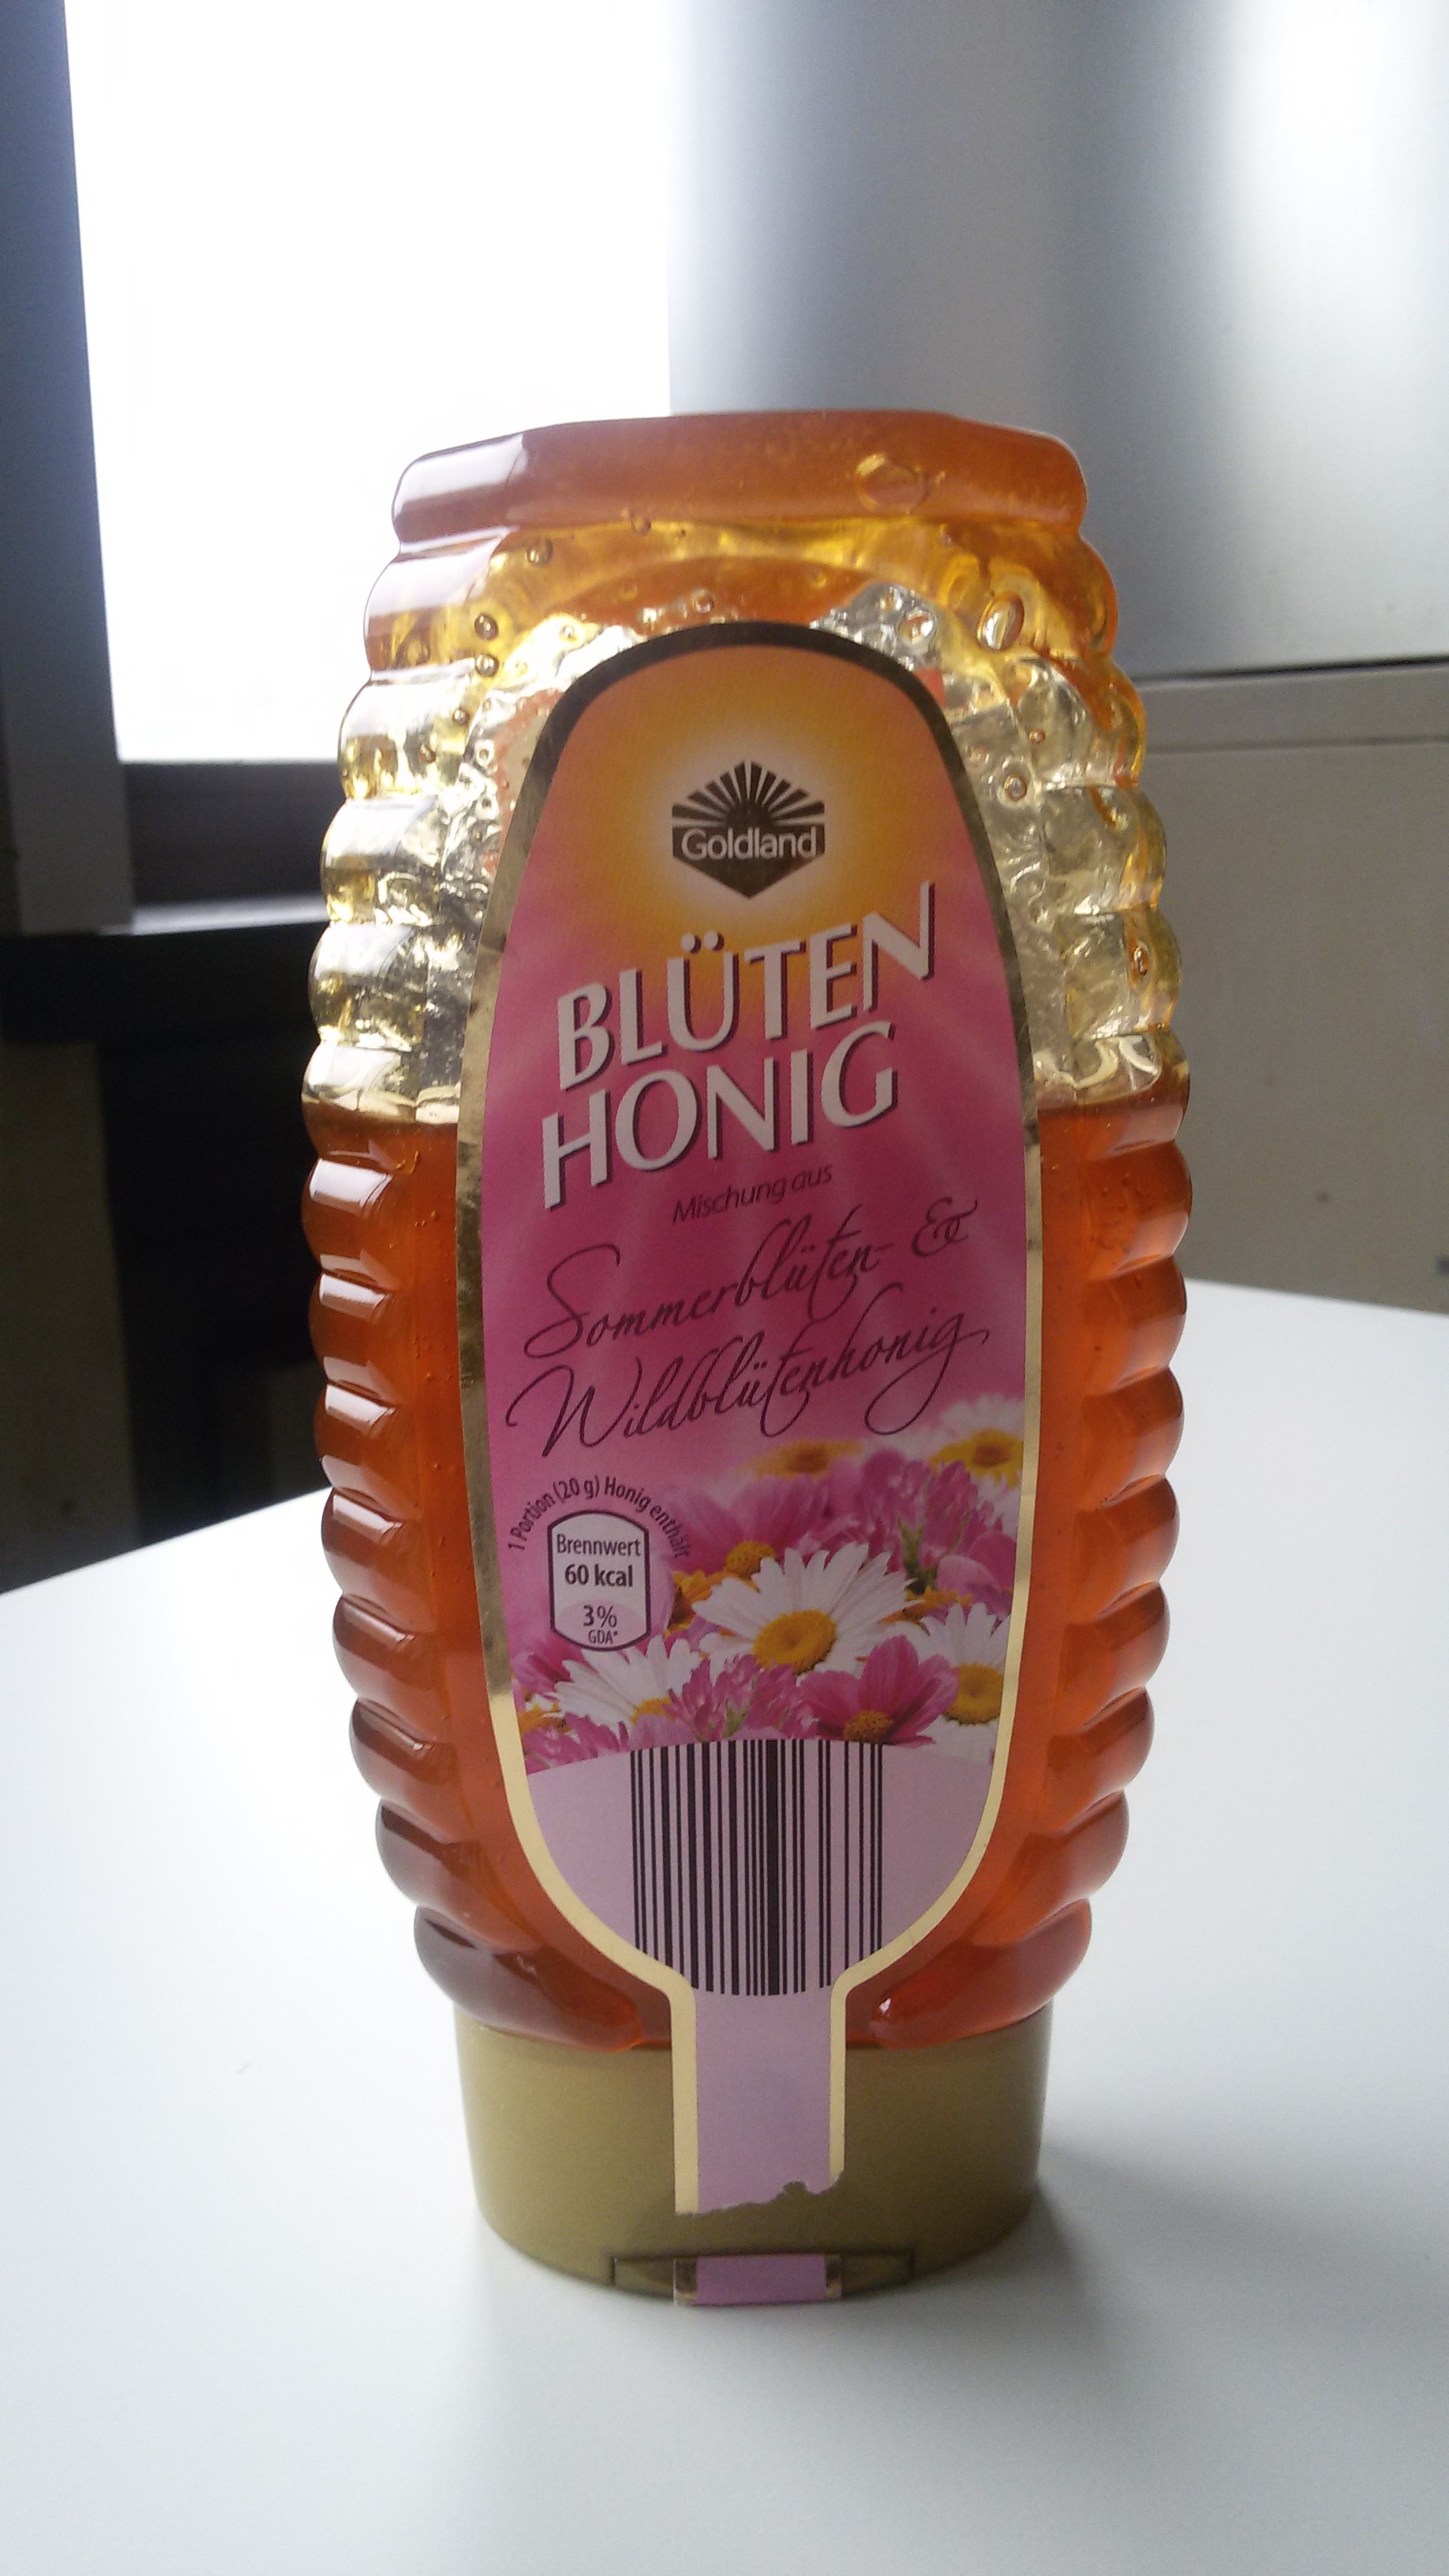
\includegraphics[]{../Bilder/20150416_182012.jpg}
  }
  \subfigure[Rückseite]{
    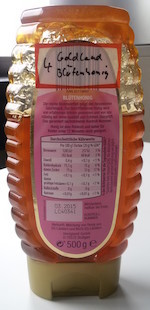
\includegraphics{../Bilder/20150416_182004.jpg}
  }
  \caption{Blütenhonig Goldland}
  \label{fig:Blütenhonig}
\end{figure}

Der Invertzucker überraschte mit seinem hohen HMF-Gehalt von ca. 300mg/kg. Dies erklärt sich durch sein Herstellungsverfahren bei dem eine Saccharoselösung mit Zitronensäure gekocht wird.\\
Der Sommerblütenhonig der Firma ''Vom Land'' (Probe 3 \ref{tab:Messergebnisse}) zeigt den höchsten HMF-Gehalt mit ca. 30mg/kg. Die Probe war nahe dem Verfallsdatum, hatte dieses aber noch nicht überschritten.\\
Der thermische Einfluss auf die Honige führte zu einem deutlichen Anstieg des HMF-Gehalts. Die Konzentrationen bewegten sich bei allen Honigen bei ca. 250mg/kg. Da alle Honige für die gleiche Zeitspanne temperiert wurden, kann man annehmen, dass die Entstehungsrate von HMF bei allen Proben annähernd identisch ist. Eine Ausnahme bildet der Sommerblütenhonig, bei dem der HMF-Gehalt mit 379mg/kg außerhalb des linearen Messbereichs liegt. Somit kann keine exakte Aussage über die HMF Bildung in der Probe 3 getroffen werden. Allerdings korreliert dieser hohe Wert mit dem gefunden HMF-Gehalt in der unbehandelten Probe 3.\\
Das Winterfutter wies einen äußerst niedrigen HMF-Gehalt auf. Dies zeigt, dass der Imker in der Winterphase den Bienenstock nicht zusätzlich erwärmt hat. Das Wärmen erniedrigt den Energieaufwand, den die Bienen im Winter erbringen müssen um ihren Stock warm zu halten. Höhere Temperaturen im Stock führen zu einem frühen Brüten der Bienen.\\
Vergleicht man die über die Kalibrierung ermittelten Werte mit den über den Festfaktor berechneten, so zeigt sich das die berechneten Werte höher sind. Die Ursache hierfür ist wahrscheinlich ein systematischer Fehler, da die Kalibriergerade mit einem Bestimmtheitsmaß von 0,9997 in sich schlüssig ist. Der Grund dafür könnte sein, dass nicht alle Matrixbestandteile bei der Fällung und anschließender Filtration abgetrennt werden konnten.\\
Eine verwendbare Kalibriergerade konnte erst im zweiten Versuch erstellt werden. Beim ersten Vermessen der Kalibrierlösungen wurde nicht die enorme Zerfallsrate des Farbkomplexes berücksichtigt. Nach WINKLER besteht nur ein Zeitfenster von einer Minute um die Messung durchzuführen.~\cite{Winkler} Die nicht verwendete Kalibriergerade ist im Anhang hinzugefügt.\\
Der Rübensirup der Firma ''Grafschafter'' (Probe 8) war nicht zur Vermessung geeignet. Zum einen war die Eigenfärbung dunkelbraun bis tiefschwarz. Eine Lichtdurchlässigkeit war unwahrscheinlich. Bei der Filtration setzten sich die Poren des Filters sofort zu. Es konnte kein Filtrat gewonnen werden.\\
\begin{figure}[htbp]
  \centering
  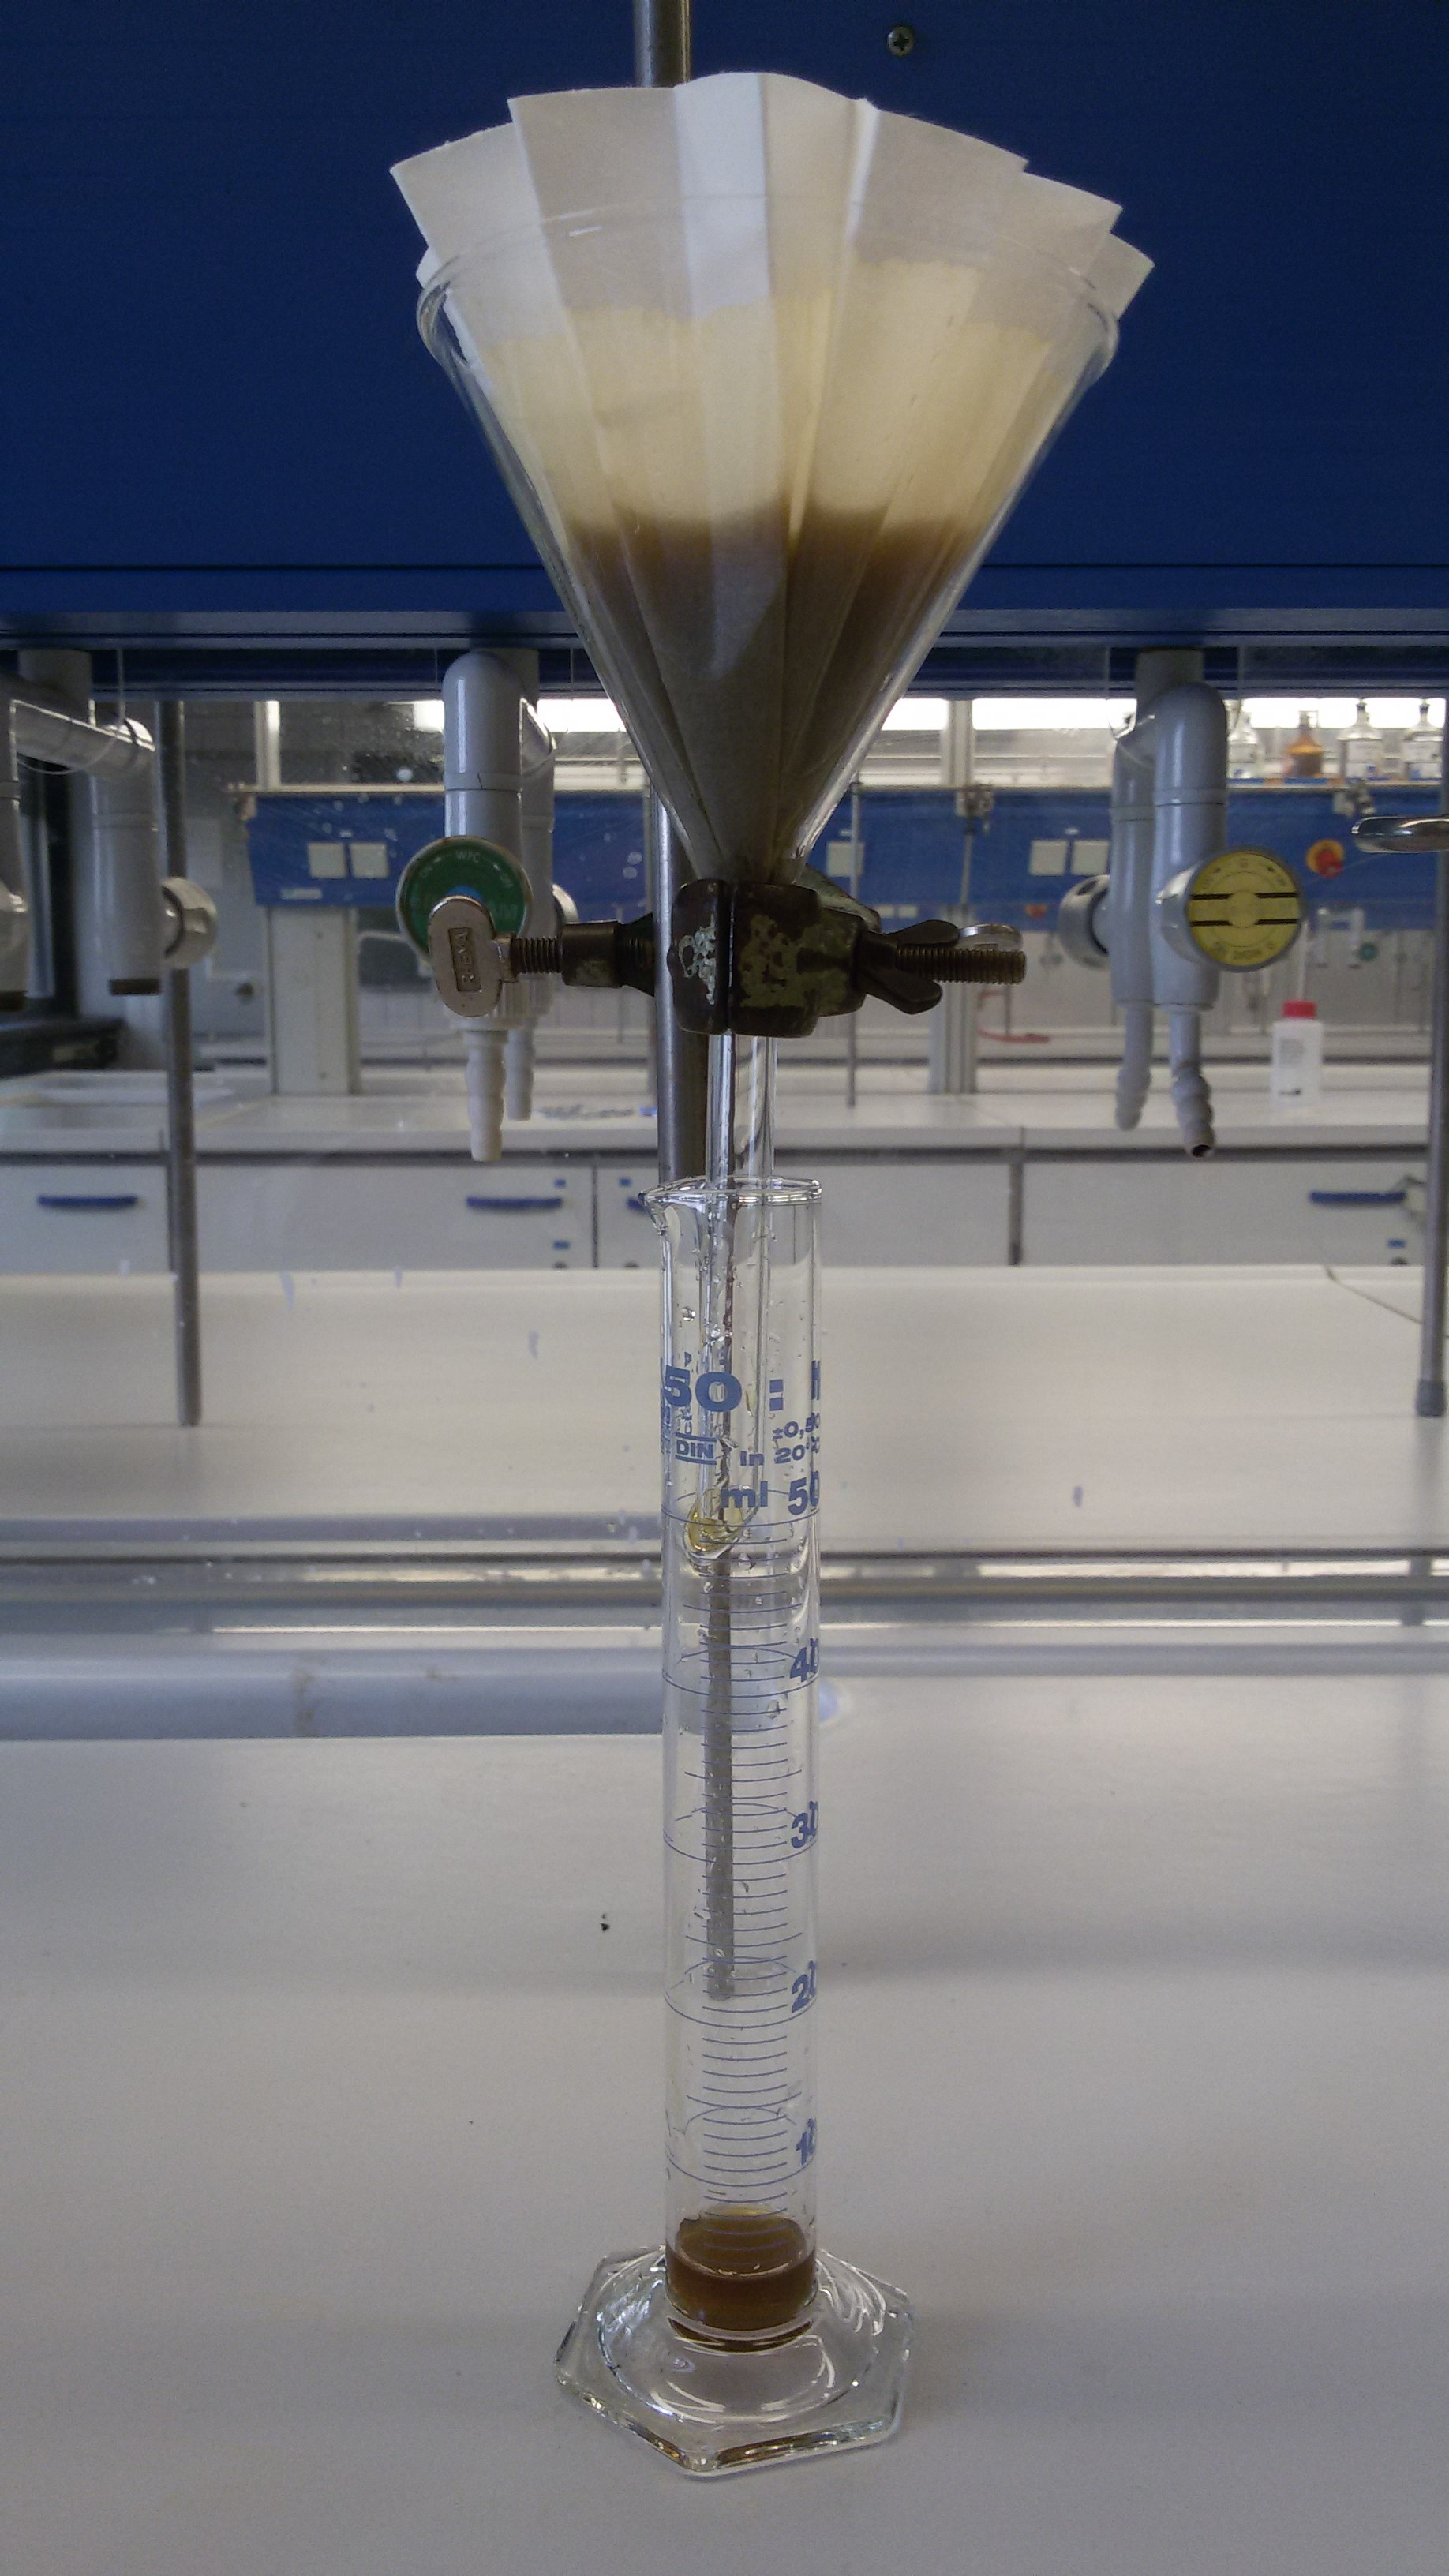
\includegraphics[width=1.00\textwidth]{../Bilder/20150427_153416.jpg}
  \caption{Filtrationsversuch Grafschafter}
  \label{fig:Grafschafter}
\end{figure}
Die durchgeführten Versuche zeigen einen ersten Einblick in das Zusammenwirken von Fruchtzucker und HMF bei thermischer Belastung, sowie bei Raumtemperatur. Zahlreiche Einflussfaktoren blieben bei den Versuchen jedoch bislang unberücksichtigt. So liegen keine Erkenntnisse über den Zusammenhang von pH-Wert, Wassergehalt und Enzymtätigkeit mit der Bildung von HMF vor. Außerdem ist nicht bekannt, ob der gesamte Fruchtzucker in Honig zu HMF umgewandelt werden kann, oder ob sich bei hoher Konzentration ein Gleichgewicht einstellt. Hierfür müssten weitere Untersuchungen, auch über einen längeren Zeitraum, durchgeführt werden.
%tropischer Honig nicht auffällig

\chapter{Exemplarische Vorschrift}

\newpage
\textbf{Danksagung}\\
\\
Zunächst möchten wir uns bei all denjenigen bedanken, die uns während der Durchführung dieses Abschlussprojektes unterstützt und motiviert haben. \\
\\
Ganz besonderer Dank gilt unseren Ehepartnern für ihre Belastbarkeit und Rücksichtnahme während der letzten vier Jahre, sowie während diesem Projekt.\\
Ebenso gilt dieser Dank unserem betreuenden Lehrer Herrn Dr. Peiter, sowie Frau Rees für ihre Hilfestellung während des praktischen Teils unseres Projektes.\\
Auch möchten wir uns bei Michael bedanken für die Bereitstellung des Originalartikels über die HMF-Bestimmung nach WINKLER und bei Herrn Dr. Seeber für die Hilfe bei der Beschaffung und Ausfuhr der Reagenzien aus der BASF.\\
Abschließend bedanken wir uns bei Benjamin ''Benni'' Hahl für die vielen Informationen über das Imkern, das Stückchen Winterfutter und bei seinen Bienen für ihren Sanftmut beim Fotografieren.


\listoffigures
\listoftables
\listofdiagrams

\bibliographystyle{gerunsrt}
\bibliography{Quellen}


\newpage


\vspace*{2cm}
\textbf{Erklärung} \\
\\
Laut §  7  Abschnitt  4  der  Fachschulverordnung für  in  modularer Organisationsform geführte 
Bildungsgänge in den Fachbereichen Technik, Wirtschaft, Gestaltung sowie Ernährung und 
Hauswirtschaft  vom  27.  Januar  2004  erklären  wir,  dass  wir  die  vorliegende  Projektarb
eit 
selbstständig und ohne fremde Hilfe verfasst haben und keine anderen als die angegebenen 
Hilfsmittel  verwendet  haben.  Alle  wörtlichen  und  sinngemäßen  Übernahmen  aus  anderen 
Werken haben wir als solche kenntlich gemacht. 

\vspace*{50pt}Sabine Klein \quad Christian Rasch



\end{document}
